\chapter[Desenvolvimento]{Desenvolvimento}

\section{Solu\c{c}\~oes Propostas}

\subsection{Planejamento de ilumina\c{c}\~ao}

Usando estruturas e materiais que al\'em de terem um baixo consumo de energia e pouco impacto ambiental em sua instala\c{c}\~ao possuem efici\^encia suficiente para atender as demandas por seguran\c{c}a da regi\~ao e dos usu\'arios do parque. Esta se mostrou a melhor proposta para  inibir atividades criminosas no local no per\'iodo da noite. Pois, iluminando o local e consequentemente as localidades pr\'oximas \`a sensa\c{c}\~ao de seguran\c{c}a ser\'a maior para os usu\'arios do parque (principalmente os praticantes de esportes) al\'em de inibir pr\'aticas il\'icitas dentro e nas imedia\c{c}\~oes da \'area iluminada.

\subsection{Planejamento ou projeto de monitoramento}

Procurar parceria com a pol\'icia militar da cidade do Gama ou de algum \'org\~ao p\'ublico que est\'a respons\'avel pela manuten\c{c}\~ao da ordem p\'ublica, com possibilidade de contrata\c{c}\~ao de uma empresa privada, al\'em de claro uma nova log\'istica de monitoramento interno com utiliza\c{c}\~ao de estruturas est\'aticas e moveis respectivamente, com a intercomunica\c{c}\~ao entre cada vi\'es de monitoramento (interno e externo), determinar um hor\'ario de funcionamento do parque e fech\'a-lo ap\'os esse per\'iodo para evitar crimes (entre eles ambientais) dentro do terreno do parque, colaborando assim com um bom funcionamento do parque, aumentar a movimenta\c{c}\~ao al\'em de ajudar a diminuir a criminalidade nas imedia\c{c}\~oes da \'area, preservando a integridade do parque e da popula\c{c}\~ao pr\'oxima. Contratar uma empresa para que sejam feita a manuten\c{c}\~ao constante do cercamento. Para que se tenha uma manuten\c{c}\~ao constante do parque \'e necess\'ario integrar empresas p\'ublicas e privadas, dessa forma \'e poss\'ivel garantir que todos os setores do parque recebam a devida manuten\c{c}\~ao, seja em uma \'area mais comum como, por exemplo, encanamento e distribui\c{c}\~ao de \'agua que pode ser feito por uma empresa p\'ublica, ou numa \'area mais espec\'ifica como a eletr\^onica de monitoramento que pode ser realizado por uma empresa privada. Utilizar empresas p\'ublicas e privadas seria a melhor op\c{c}\~ao para manter a manuten\c{c}\~ao no parque, pois existem diversos setores que necessitam de aten\c{c}\~ao. Na parte estrutural t\^em-se a manuten\c{c}\~ao do cercamento, das cal\c{c}adas ao redor do parque e do circuito de \textit{cooper} como exemplos, na parte de monitoramento, a manuten\c{c}\~ao das c\^ameras e dos softwares que fazem esse trabalho. Ou seja, seria necess\'ario ter empresas que atuam em diversas \'areas de conhecimento, isso justifica o porqu\^e de se usar empresas p\'ublicas e privadas.

\subsection{Postes com placa solar para abastecimento pr\'oprio}

Utiliza\c{c}\~ao de postes de ilumina\c{c}\~ao que possuem em sua parte superior uma placa fotovoltaica que capta a radia\c{c}\~ao solar e transforma em energia, que \'e armazenada em baterias no poste. Cada poste \'e um sistema isolado, ou seja, n\~ao conectado com a rede, sendo assim, uma falha em um deles n\~ao afeta os outros.

\subsection{Turbinas de vento para gera\c{c}\~ao de energia el\'etrica.}

A energia e\'olica - produzida a partir da for\c{c}a dos ventos - \'e abundante, renov\'avel, limpa e dispon\'ivel em muitos lugares. Essa energia \'e gerada por meio de aerogeradores, nas quais a for\c{c}a do vento \'e captada por h\'elices ligadas a uma turbina que aciona um gerador el\'etrico. A quantidade de energia transferida \'e em fun\c{c}\~ao da densidade do ar, da \'area coberta pela rota\c{c}\~ao das p\'as (h\'elices) e da velocidade do vento. \\ 

A avalia\c{c}\~ao t\'ecnica do potencial e\'olico exige um conhecimento detalhado do comportamento dos ventos. Os dados relativos a esse comportamento - que auxiliam na determina\c{c}\~ao do potencial e\'olico de uma regi\~ao - s\~ao relativos \`a intensidade da velocidade e \`a dire\c{c}\~ao do vento. Para obter esses dados, \'e necess\'ario tamb\'em analisar os fatores que influenciam o regime dos ventos na localidade do empreendimento. Entre eles pode-se citar o relevo, a rugosidade do solo e outros obst\'aculos distribu\'idos ao longo da regi\~ao. \\ 

Para que a energia e\'olica seja considerada tecnicamente aproveit\'avel, \'e necess\'ario que sua densidade seja maior ou igual a 500 W/m$^{2}$, a uma altura de 50 metros, o que requer uma velocidade m\'inima do vento de 7 a 8 m/s (GRUBB; MEYER,1993). Segundo a Organiza\c{c}\~ao Mundial de Meteorologia, o vento apresenta velocidade m\'edia igual ou superior a 7 m/s, a uma altura de 50 m, em apenas 13\% da superf\'icie terrestre. Essa propor\c{c}\~ao varia muito entre regi\~oes e continentes. \\

Quanto \`a aplica\c{c}\~ao desse tipo de energia no Brasil, pode-se dizer que as grandes centrais e\'olicas podem ser conectadas \`a rede el\'etrica uma vez que possuem um grande potencial para atender o Sistema Interligado Nacional (SIN). As pequenas centrais, por sua vez, s\~ao destinadas ao suprimento de eletricidade a comunidades ou sistemas isolados, contribuindo para o processo de universaliza\c{c}\~ao do atendimento de energia. Em rela\c{c}\~ao ao local, a instala\c{c}\~ao pode ser feita em terra firme (\textit{on-shore}) ou no mar (\textit{off-shore}). \\ 

O Atlas do Potencial E\'olico Brasileiro, elaborado pelo Centro de Pesquisas de Energia El\'etrica (Cepel), mostra um potencial bruto de 143,5 GW, o que torna a energia e\'olica uma alternativa importante para a diversifica\c{c}\~ao do "mix" de gera\c{c}\~ao de eletricidade no Pa\'is. O maior potencial foi identificado na regi\~ao litoral do Nordeste e no Sul e Sudeste. O potencial de energia anual para o Nordeste \'e de cerca de 144,29 TWh/ano; para a regi\~ao Sudeste, de 54,93 TWh/ano; e, para a regi\~ao Sul, de 41,11 TWh/ano. \\

\subsubsection{Impactos de uso}

Os equipamentos de pequeno porte t\^em impacto ambiental geralmente desprez\'ivel. J\'a os impactos ambientais de parques e\'olicos podem ser classificados em:

\begin{itemize}
     \item Uso da terra: em parques e\'olicos as turbinas devem estar suficientemente distanciadas entre si para evitar a pertuba\c{c}\~ao causada no escoamento do vento entre uma unidade a outra. Estes espa\c{c}amentos devem ser no m\'inimo de 5 a 10 vezes a altura da torre. Contudo a \'area do parque pode ser aproveitada para produ\c{c}\~ao agr\'icola  ou atividades de lazer
     \item Ru\'ido - as turbinas de grande porte geram ru\'ido aud\'ivel significativo, de forma que existe regulamenta\c{c}\~ao relativa \`a sua instala\c{c}\~ao na vizinhan\c{c}a de \'areas residenciais. Entretanto, nas turbinas mais modernas o n\'ivel de barulho tem sido reduzido. O ru\'ido \'e proveniente de duas fontes: o pr\'opio fluxo de ar nas p\'as e os mecanismos (gerador, caixa de redu\c{c}\~ao)
     \item Impactos visuais - as p\'as das turbinas produzem sombras e/ou reflexos m\'oveis que s\~ao indesej\'aveis nas \'areas residenciais; este problema \'e mais evidente em pontos de latitudes elevadas, onde o sol tem posi\c{c}\~ao mais baixa no c\'eu. Dentre outros par\^ametros que se podem relacionar s\~ao: o tamanho da turbina, seu design, n\'umeros de p\'as, cor e n\'umeros de turbinas em uma fazenda e\'olica. As m\'aquinas de grande porte s\~ao objetos de muita visibilidade e interferem significativamente nas paisagens naturais; por isso podem existir restri\c{c}\~oes \`a sua instala\c{c}\~ao em algumas \'areas (por exemplo, em \'areas tur\'isticas ou \'areas de grande beleza natural);
	\item Aves - em fazendas \'eolicas ocorre mortalidade de aves por impacto com as p\'as das turbinas (acredita-se que os animais n\~ao conseguem enxerg\'a-las, quando est\~ao em movimento), por isso n\~ao \'e recomend\'avel a sua instala\c{c}\~ao em \'areas de migra\c{c}\~ao de aves, \'areas de reprodu\c{c}\~ao e \'areas de prote\c{c}\~ao ambiental.
        \item Interfer\^encia eletromagn\'etica - esta acontece quando a turbina e\'olica \'e instalada entre os receptores e transmissores de ondas de r\'adio, televis\~ao e microondas. As p\'as das turbinas podem refletir parte da radia\c{c}\~ao eletromagn\'etica em uma dire\c{c}\~ao, tal que a onda refletida interfere no sinal obtido.
	\end{itemize}

\subsubsection{Viabilidade econ\^omica} 

Conforme j\'a mencionado  n\~ao \'e considerado vi\'avel, a implanta\c{c}\~ao de parque e\'olicos em \'areas urbanas, pois esses locais  apresentam rugosidade bastante elevada (em geral, quanto mais acentuada a rugosidade da superf\'icie da terra, mais o vento ser\'a abrandado), de forma que os ventos pr\'oximos \`a superf\'icie s\~ao fracos e muito turbulentos. \\ De uma forma geral, os sistemas e\'olicos s\~ao bastante dur\'aveis e precisam de pouca manuten\c{c}\~ao. A vida \'util das turbinas e\'olicas \'e estimada em 15 anos. Os dispositivos eletr\^onicos (inversor, controlador de carga) t\^em vida \'util superior a 10 anos. No caso de sistemas e\'olicos isolados com armazenamento de energia em baterias, as baterias s\~ao consideradas o ponto cr\'itico do sistema, mas quando este \'e bem projetado elas t\^em vida \'util de 4 a 5 anos. \\ As turbinas modernas s\~ao projetadas para funcionar por 130 mil horas de opera\c{c}\~ao, o que resulta em uma vida \'util em torno de vinte anos. Seu custo de instala\c{c}\~ao est\'a situado por volta de US\$ 1.500.000 por cada MW da capacidade instalada. As experi\^encias internacionais t\^em mostrado que o custo de manuten\c{c}\~ao \'e geralmente muito baixo para turbinas novas e aumenta um pouco com o tempo de funcionamento das mesmas. Para m\'aquinas novas, estima-se um custo anual entre 1,5 a 2\% do investimento, enquanto as turbinas com mais idade apresentam um custo em torno de 3\% ao ano do investimento. \\

\subsubsection{Viabilidade da Energia E\'olica no parque do Gama}

Um estudo das velocidades dos ventos no DF realizado pela (Universidade de Bras\'ilia - Bras\'ilia, DF), durante os meses do ano no per\'iodo de 2000 a 2010, demonstrou n\~ao ser imediatamente vi\'avel a implanta\c{c}\~ao de uma usina e\'olica no local, pois, a velocidade do vento m\'edia anual foi de 1,46 m/s, sendo que a velocidade do vento m\'edia \`a noite foi 48\% menor do que durante o dia. Para que a energia e\'olica seja considerada tecnicamente aproveit\'avel, \'e necess\'ario que sua densidade seja maior ou igual a 500 W/m$^{2}$, a uma altura de 50 metros, o que requer uma velocidade m\'inima do vento de 7 a 8 m/s. 
Uma an\'alise de frequ\^encia das medi\c{c}\^oes para cada m\^es do ano foi utilizada para definir a dire\c{c}\~ao predominante do vento diurno e noturno. Os resultados indicam que \`a noite, durante todo o ano, os ventos foram predominantemente S e SE, enquanto que durante o dia a predomin\^ancia foi de ventos NE e E, exceto para o m\^es de dezembro, quando o vento predominante foi N. \\

A dire\c{c}\~ao do vento n\~ao apresentou predomin\^ancia muito definida quando os dados foram analisados para as 24 h do dia, por\'em quando analisados separadamente para os per\'iodos diurnos e noturnos, foi poss\'ivel distinguir diferen\c{c}as. Para todos os meses do ano ocorreu uma maior frequ\^encia de ventos de nordeste - NE (Jan a Mai, Out e Nov), e leste - E (Jun a Set) durante o per\'iodo diurno, com exce\c{c}\~ao do m\^es de Dezembro, quando a maior frequ\^encia foi de ventos de norte - N. Durante o per\'iodo noturno, a maior frequ\^encia de ventos de sul - S ocorreu nos meses de Abril a Julho, enquanto que para os outros meses a maior frequ\^encia foi de ventos de sudeste - SE. \\

O valor m\'aximo de velocidade do vento durante o per\'iodo foi U$_{max}$ = 14,49 m/s, observado no m\^es de Outubro, e sua dire\c{c}\~ao foi de oeste - W. Mesmo apresentado um grande potencial de escoamento de ventos durante um per\'iodo do ano, a efici\^encia da produ\c{c}\~ao de energia e\'olica precisaria ser melhor estudada, pois a localiza\c{c}\~ao de um Parque e\'olico dentro de um centro urbano n\~ao \'e considerado vi\'avel, pois esses locais  apresentam rugosidade bastante elevada (em geral, quanto mais acentuada a rugosidade da superf\'icie da terra, mais o vento ser\'a abrandado, al\'em das edifica\c{c}\^oes que dificultam a passagem dos ventos), de forma que os ventos pr\'oximos \`a superf\'icie s\~ao fracos e muito turbulentos.

\subsection{Sistema de capta\c{c}\~ao e reutiliza\c{c}\~ao da \'agua da chuva.}

Normalmente a \'agua \'e drenada atrav\'es da rede pluvial para os rios e c\'orregos, por\'em uma boa alternativa pode ser seu reaproveitamento em processos industriais e vasos sanit\'arios. As calhas e condutores horizontais e verticais s\~ao os que recebem toda a \'agua captada pelo telhado, estas dever\~ao obedecer \`as normas brasileiras de instala\c{c}\~ao de esgoto pluvial (NBR - 10.844/89) da ABNT.
Um sistema simples de capta\c{c}\~ao de \'agua pluvial com calhas que direcionam a \'agua da chuva para um filtro seletor que ir\'a separar os res\'iduos s\'olidos como folhas e impurezas que ficam nas calhas, despejando a \'agua filtrada em um reservat\'orio inferior (cisterna) para o armazenamento pode ser uma \'otima op\c{c}\~ao.

\subsection{Placas solares em cima de edifica\c{c}\~oes.}

 A energia solar \'e considerada uma fonte de energia inesgot\'avel. Pode-se falar que \'e uma fonte de energia promissora. Indiretamente, o sol tem uma participa\c{c}\~ao em quase todas outras fontes de energia. A evapora\c{c}\~ao, por exemplo, acontece por causa do sol, a origem das \'aguas para os represamentos etc. A radia\c{c}\~ao solar tamb\'em induz a circula\c{c}\~ao atmosf\'erica em larga escala, causando os ventos. Petr\'oleo, carv\~ao e g\'as natural foram gerados a partir de res\'iduos de plantas e animais que, originalmente, necessitam da energia solar \cite{CRESESB}. \\ 
 
 Lembrando que essa \'e uma an\'alise preliminar, pois n\~ao foram coletados dados de consumo el\'etrico da regi\~ao estudada. Tendo isso em mente, ser\'a calculado quanto de energia pode ser gerada na \'area dispon\'ivel acima de edifica\c{c}\^oes. 
 
 \subsubsection{An\'alise de viabilidade}
 
 Edifica\c{c}\^oes e suas respectivas \'areas:
 
 \begin{itemize}
        \item Sede Administrativa			125,97m$^{2}$
	\item Quiosque Comercial			64,97m$^{2}$
	\item Guaritas				22,77m$^{2}$
	\item Conjuntos de banheiros p\'ublicos	58,60m$^{2}$
	\item Torre de vigil\^ancia			33,70m$^{2}$
\end{itemize}

TOTAL					306,01m$^{2}$\\

A efici\^encia de produ\c{c}\~ao por um painel solar \'e dita em quanto de energia luminosa provida pelo sol na \'area de 1m$^{2}$ que ela converte em eletricidade, em porcentagem. Para pain\'eis fotovoltaicos de Sil\'vicio cristalino (os pain\'eis mais utilizados no mercado), a efici\^encia comercial vai de 13\% a 16\%, sendo que quando a efici\^encia indicada for maior que 16\% ele \'e considerado uma placa fotovoltaica (premium). Para base de c\'alculo, ser\'a utilizada efici\^encia de 15\%. \\

A partir de uma consulta no site do CRESESB, foram encontrados os valores indicados na figura abaixo, dentre os quais, utilizaremos o menor valor da linha - Maior m\'inimo mensal -, pois teremos assim uma baixa expectativa, que tende a ser superada.

\begin{figure}[h]
	\centering
	\label{Calculo Plano Inclinado}
		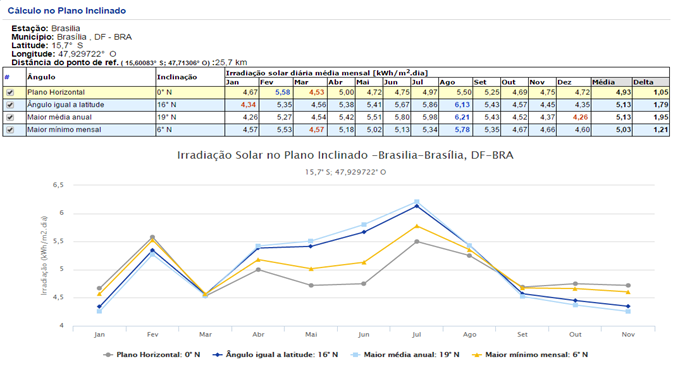
\includegraphics[keepaspectratio=true,scale=0.7]{figuras/CalculoPlanoInclinado.png}
	\caption{Dados Solarim\'etricos de Bras\'ilia}
	\small{Fonte:  <http://www.cresesb.cepel. br/index.php?section=sundata>}
\end{figure}

Utilizando ent\~ao placas de 15\% de efici\^encia em um local que o \'indice solarim\'etrico \'e de 4,57 kWh/m$^{2}$.dia temos que a energia el\'etrica gerada por metro quadrado de placa fotovoltaica em um dia \'e de 685,5 Wh Ent\~ao, em uma \'area de 306,01m$^{2}$ e no per\'iodo de 30 dias seria gerado 6293,1 kWh. Como \'e improv\'avel que 100\% da \'area seja aproveitada, ser\'a descontado 20\% para melhorar a estimativa, que fica 5034,5 kWh. Como a ilumina\c{c}\~ao do parque envolve postes que geram sua pr\'opria energia, tamb\'em com placas solares, essa energia seria utilizada para alimentar a ilumina\c{c}\~ao interna, e pequenos eletrodom\'esticos, e caso haja excedente, redistribu\'ida na rede el\'etrica para a comunidade.

Com isso conclui-se que sem impactos ambientais, e sem a necessidade de construir outras estruturas, a quantidade de energia gerada por pain\'eis fotovoltaicos instalados apenas sobre as edifica\c{c}\^oes m\'inimas do edital de licita\c{c}\~ao, \'e suficiente para abastecer at\'e 30 resid\^encias, admitindo o valor m\'edio de 167 kWh por resid\^encia (Relat\'orio da EPE - Empresa de Pesquisa Energ\'etica). Com isso \'e aceit\'avel dizer que \'e suficiente para abastecer o parque.

\subsection{Coleta Seletiva}

Reduzir, reutilizar e reciclar. \'E com base nesses tr\^es princ\'ipios que percebeu-se a import\^ancia e a viabilidade de se implantar o Programa de Gerenciamento de Res\'iduos S\'olidos (PGRS) no parque urbano da cidade do Gama-DF. Tendo como base a sua implanta\c{c}\~ao no parque tem\'atico Beto Carrero World em Santa Catarina no primeiro semestre de 2013. Essa iniciativa faz com que o cuidado com o meio ambiente seja feito por meio do reaproveitamento de materiais atrav\'es da reciclagem. \\
O programa prev\^e que \'e responsabilidade todos, separar os res\'iduos, desde o funcion\'ario at\'e o visitante. O programa funciona de forma que torna-se comum o visitante do parque se deparar com duas lixeiras, uma laranja, para res\'iduo recicl\'avel e outra cinza, destinada ao res\'iduo n\~ao recicl\'avel, como por exemplo, os org\^anicos. Al\'em das cores das lixeiras, tamb\'em s\~ao utilizados cores diferentes de sacos de lixo. Desta forma quando os res\'iduos chegam aos bastidores, j\'a se sabe o tipo de res\'iduos e a forma/local de armazenamento.

\subsection{L\^ampadas de LED}

\subsection{Solu\c{c}\~ao de servi\c{c}os}

Espa\c{c}o lazer multim\'idia, que traga alguma forma de moderniza\c{c}\~ao tecnol\'ogica que torne interessante a realiza\c{c}\~ao de eventos no Parque do Gama

\subsection{Esportes}

Uma op\c{c}\~ao vi\'avel seria a bicicleta ergom\'etrica que armazene energia para iluminar uma quadra. Entretanto a quest\~ao da viabilidade econ\^omica e de gera\c{c}\~ao de energia foi questionada pelo grupo e nesse sentido pensou-se em uma alternativa de bicicleta (m\'ovel) que tenha uma tecnologia embarcada que mostre em tempo real, dados espec\'ificos do rendimento metab\'olico daquela atividade, podendo ser transmitido para um aplicativo para smartphone/tablet.

\subsubsection{Estudo da viabilidade}

Wi-Fi Comunit\'ario: Esse projeto, demanda um custo alto de acordo com a quantidade de totens a serem instalados no parque. Estimando um valor pr\'oximo ao valor que a Prefeitura de S\~ao Paulo paga por seus pontos de acesso Wifi em pra\c{c}as, ficaria em torno de R\$ 6500,00 por m\^es por \'areas com ponto de acesso, mais os custos iniciais com a instala\c{c}\~ao, considerando que o Parque do Gama tenha \'area correspondente \`a 10 pra\c{c}as da cidade S\~ao Paulo, o custo seria aproximadamente R\$ 65000,00 por m\^es, logo etorno de R\$ 780000,00 ao ano. Um custo vi\'avel, caso o projeto consiga o apoio do Governo do Distrito Federal e/ou empresas patrocinadoras. \\ O uso de bicicletas ergom\'etricas sustent\'aveis \'e uma forma de produzir energia el\'etrica limpa. Ela pode ser estacionada ou m\'ovel. Seria uma maneira atrativa, para incentivar os frequentadores do parque a praticarem exerc\'icios com ajuda na concientiza\c{c}\~ao ambiental. Essas bicicletas usadas em grande escala, podem gerar a energia necess\'aria para a ilumina\c{c}\~ao das quadras poli-esportivas por exemplo. Quando m\'ovel, poderia existir um aplicativo de celular para saber quantas calorias, est\~ao sendo perdidas. Essas bicicletas estacionadas j\'a est\'a sendo de grande uso em academias e grandes hot\'eis, pois produz energia el\'etrica de forma limpa.

\subsection{Infraestrutura}

Rede Wifi comunit\'aria (o sinal de Wifi ser\'a gratuito e de livre acesso, sem necessidade de cadastro, tendo como exemplo o projeto Pra\c{c}as Wifi Livre SP, projeto que j\'a est\'a em funcionamento na cidade de S\~ao Paulo, onde a prefeitura instalou pontos de transmiss\~ao Wifi gratuitos, com velocidade e 512kbit/s , em v\'arias pra\c{c}as, a adapta\c{c}\~ao que pode ser feita no Parque do Gama, \'e que esses pontos de acesso sejam em totens, com tomadas e cabos para carregar os celulares, tablets e notebooks, como os j\'a utilizados em v\'arios shoppings, e velocidade da internet seja de ao menos 1 mega. E esses totens seriam localizados em \'areas de maior movimenta\c{c}\~ao do parque). 

\section{Solu\c{c}\~oes Adotadas}

\subsection{Capta\c{c}\~ao de \'aguas pluviais}

No Brasil, o sistema para capta\c{c}\~ao de \'agua \'e utilizado em algumas cidades do Nordeste como fonte de suprimento devido aos per\'iodos de seca. A viabilidade do uso de \'agua da chuva \'e caracterizada pela diminui\c{c}\~ao da demanda de \'agua fornecida por companhias de saneamento, gerando assim uma economia de custos com a \'agua e redu\c{c}\~ao de reten\c{c}\~ao da mesma em locais que possam causar enchentes. \cite{MAY} \\ Os principais objetivos da capta\c{c}\~ao e aproveitamento das \'aguas da chuva s\~ao: utiliza\c{c}\~ao nos banheiros, tanto na limpeza quanto nas descargas de vasos sanit\'arios; utilizados na irriga\c{c}\~ao dos jardins na \'epoca de seca; evitando ac\'umulo de \'agua em locais com depress\~ao, por captar a \'agua e canaliz\'a-la para um reservat\'orio. \\ No processo de capta\c{c}\~ao da \'agua s\~ao utilizadas \'areas imperme\'aveis, como por exemplo, os telhados. Este projeto visa a disponibiliza\c{c}\~ao da coleta da \'agua nos telhados dos banheiros, da administra\c{c}\~ao e das torres de seguran\c{c}a. Nos locais que tiver certa inclina\c{c}\~ao, ser\~ao colocadas calhas capazes de canalizar a \'agua e lev\'a-la para os tanques, onde ser\~ao tratadas e enviadas para sua utiliza\c{c}\~ao. \cite{MAY} \\ Segundo a Leal \cite{LEAL}, o sistema de aproveitamento da \'agua da chuva funciona da seguinte maneira: a \'agua \'e coletada de \'areas imperme\'aveis e em seguida \'e filtrada e armazenada em um reservat\'orio de acumula\c{c}\~ao, que pode ser apoiado, enterrado ou elevado e pode ser constru\'ido de diferentes materiais como: concreto armado, bloco de concreto, alvenaria de tijolos, a\c{c}o, pl\'astico, poli\'ester, polietileno e outros. \\ Os par\^ametros principais envolvidos no sistema de coleta e aproveitamento da \'agua de chuva s\~ao: \'area de coleta, quantidade de \'agua a ser armazenada, qualidade da \'agua, capacidade de armazenamento e confiabilidade. \\ Para n\~ao ocorrerem entupimentos nos dutos que levam a \'agua canalizada para os tanques s\~ao usadas peneiras para retirada de folhas e galhos maiores, essas grades ser\~ao posicionadas por toda a calha aumentando um pouco o custo, por\'em evitando poss\'iveis problemas na filtragem, como pode ser observado na figura abaixo. Ser\~ao usado 122 mm x 3m dessa calha, e pode ser encontrada na Leroy Merlin a um valor de R\$ 59,90. 

\begin{figure}[h!]
	\centering
	\label{Grades usadas na calha}
		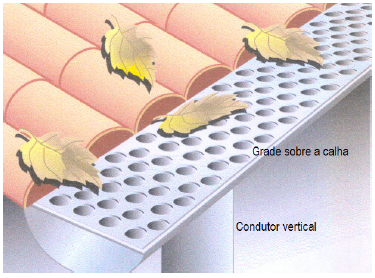
\includegraphics[keepaspectratio=true,scale=0.9]{figuras/GradesUsadasNaCalha.png}
	\caption{Grades usadas na calha}
	\small{Fonte: \cite{WATERFALL}}
\end{figure}

Os condutores, que servem para canalizar a \'agua do telhado ser\~ao as calhas com grades colocadas nas extremidades das constru\c{c}\~oes, como ilustra a Figura abaixo.

\begin{figure}[h!]
	\centering
	\label{Sistema de calhas na \'area do telhado}
		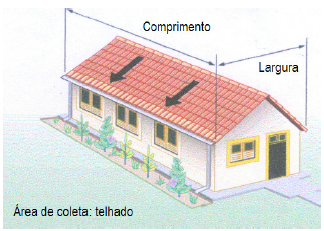
\includegraphics[keepaspectratio=true,scale=1.2]{figuras/SistemaDeCalhasNaAreaDoTelhado.png}
	\caption{Sistema de calhas na \'area do telhado}
	\small{Fonte:  \cite{WATERFALL}}
\end{figure}

O armazenamento ser\'a feito a partir do estudo de 8 tipos de tanques, devido a disponibilidade e a facilidade de constru\c{c}\~ao, para tanto foi realizado um estudo, apresentado na Tabela abaixo, da capacidade de armazenamento, viabilidade econ\^omica, e m\~ao-de-obra.

\begin{figure}[h!]
	\centering
	\label{Tipo de Tanques}
		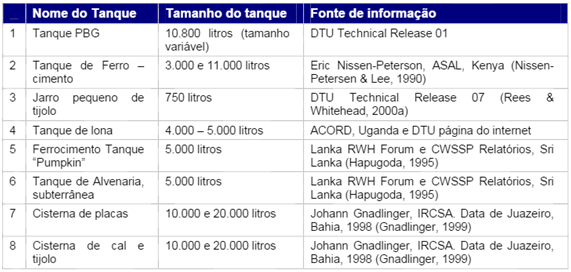
\includegraphics[keepaspectratio=true,scale=1.2]{figuras/TipoDeTanques.png}
	\caption{Tipo de Tanques}
	\small{Fonte:  \cite{TERRYTHOMAS}}
\end{figure}

\begin{figure}[h!]
	\centering
	\label{Comparativo dos Tanques}
		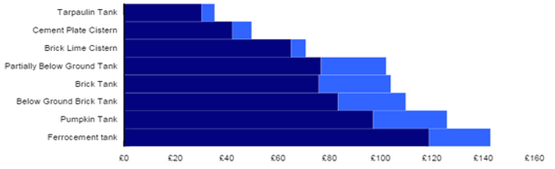
\includegraphics[keepaspectratio=true,scale=1.2]{figuras/ComparativoDosTanques.png}
	\caption{Comparativo dos Tanques}
	\small{Fonte:  \cite{TERRY THOMAS}}
\end{figure}

 Esse gr\'afico foi feito a partir da tabela acima sobre os tipos de tanques, mostrando o custo do material, a convers\~ao foi feita seguindo a cota\c{c}\~ao atual, sendo 1 libra esterlina igual a 4,36 reais. \\ Tendo em vista os tanques estudados na figura \ref{Tipo de Tanques}, o que se mostrou mais economicamente atrativo foi o "Cement Plate Cistern", a cisterna de placas cimentadas, a qual armazena de 10 mil a 20 mil litros de \'agua, o mesmo \'e melhor para o parque devido ao seu custo de opera\c{c}\~ao e instala\c{c}\~ao serem baixos, o cimento \'e barato, gerando um custo de 500 reais para a constru\c{c}\~ao. O tanque do tipo placas cimentadas segue a ideia de ser encostado na edifica\c{c}\~ao, portanto eles ser\~ao posicionados ao lado dos banheiros, guarita de seguran\c{c}a, administra\c{c}\~ao e quiosque sem consumir muito espa\c{c}o e com sinaliza\c{c}\~ao para que os usu\'arios n\~ao mexam na instala\c{c}\~ao. A Figura a seguir apresenta o sistema de capta\c{c}\~ao de \'agua a ser implantado no Parque do Gama.\cite{JOHANN} 
 
 \begin{figure}[h!]
	\centering
	\label{SistemaDeCaptacao}
		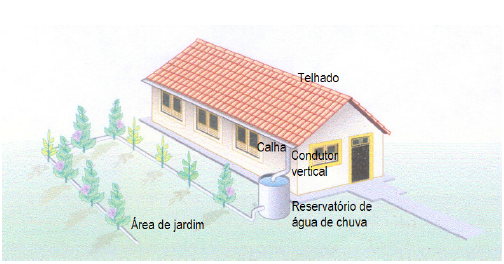
\includegraphics[keepaspectratio=true,scale=1.0]{figuras/SistemaDeCaptacao.png}
	\caption{Sistema de capta\c{c}\~ao}
	\small{Fonte:  \cite{WATERFALL}}
\end{figure}
 
 A figura abaixo mostra a quantidade de litros de \'agua em uma irriga\c{c}\~ao de acordo com o di\^ametro da mangueira, mostrando a quantidade de \'agua p\'ublica que \'e perdida com essa atividade. Sendo assim, ser\'a utilizada uma mangueira de $^{3}$/$_{4}$ polegadas por apresentar maior vaz\~ao volum\'etrica.  Por exemplo, para um uso de 15 minutos, seriam gastos 499 litros de \'agua, portanto seria aconselh\'avel o reuso da \'agua de chuva para tal atividade.
 
 \begin{figure}[h!]
	\centering
	\label{ConsumoAguaRega}
		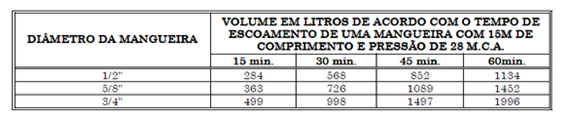
\includegraphics[keepaspectratio=true,scale=1.0]{figuras/ConsumoAguaRega.png}
	\caption{Estimativa do consumo da \'agua na torneira de jardins por tempo de rega}
	\small{Fonte:  \cite{VICKERS}}
\end{figure}
 
 Um ponto relevante a ser considerado \'e que em hip\'otese alguma a \'agua da chuva captada poder\'a ser misturada a \'agua pot\'avel. Al\'em disso, \'e necess\'ario que ocorra a limpeza da \'agua. Para isso, ser\'a usado um filtro VF1 o qual recebe a \'agua da chuva e filtra os galhos e folhas que passaram pela grade das calhas, em seguida, a \'agua passa por uma tela de malha de 0,26 mm que se localiza abaixo das ripas e \'e direcionada ao reservat\'orio. A frequ\^encia da manuten\c{c}\~ao varia conforme a incid\^encia da sujeira, ocorrendo de 1 a 2 vezes ao ano. O filtro \'e mostrado abaixo e pode ser encontrado no valor de 2100 reais. \cite{VICKERS} 
 
\begin{figure}[h!]
	\centering
	\label{SistemaDeFiltroUtilizado}
		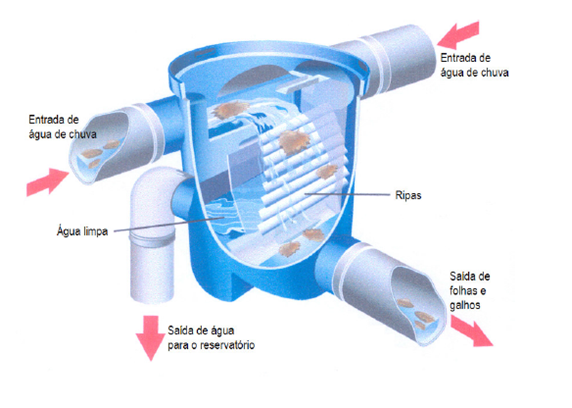
\includegraphics[keepaspectratio=true,scale=0.8]{figuras/SistemaDeFiltroUtilizado.png}
	\caption{Sistema de filtro utilizado}
	\small{Fonte:  \cite{TECHINIK}}
\end{figure}
 
 A figura a seguir apresenta o tipo da \'agua da chuva, com o filtro usado e a desinfec\c{c}\~ao requerida. No parque ser\'a utilizada \'agua n\~ao pot\'avel, pois apresenta filtros e tratamento qu\'imico com cloro, para no caso de contato com a pele, n\~ao cause nenhum efeito colateral.
 
\begin{figure}[h!]
	\centering
	\label{TipoAguaPropriedadesExigidas}
		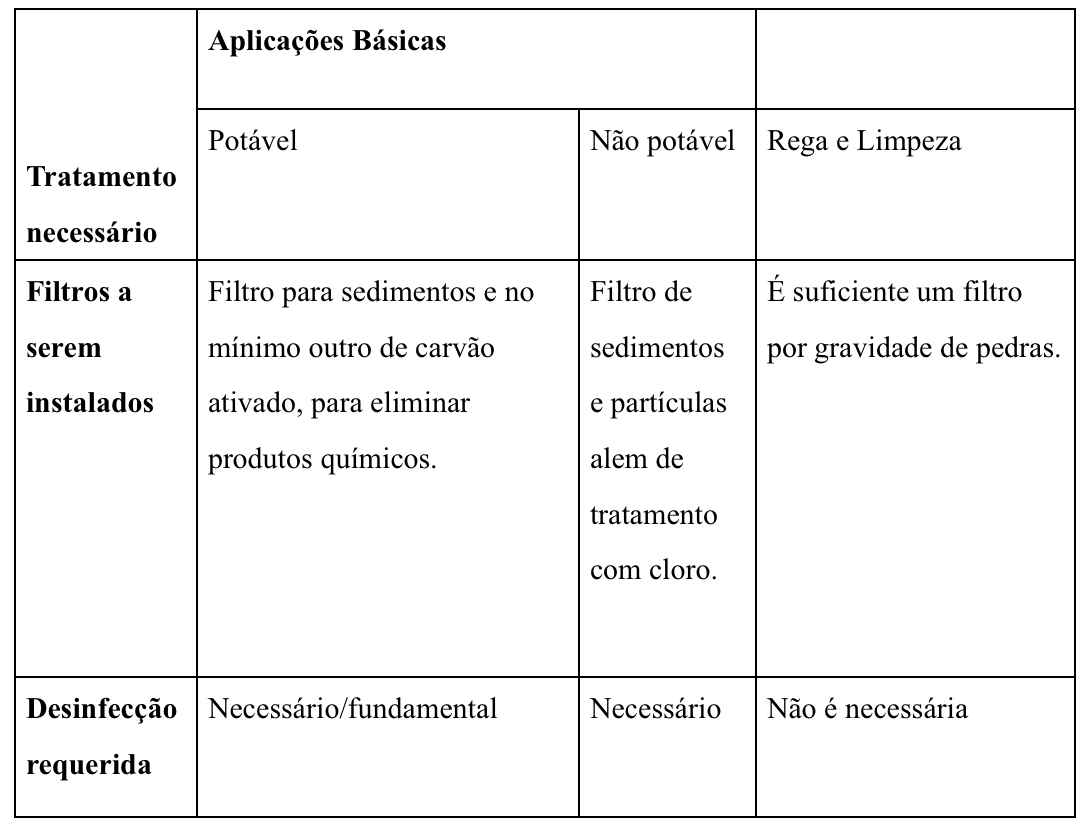
\includegraphics[keepaspectratio=true,scale=0.8]{figuras/TipoAguaPropriedadesExigidas.png}
	\caption{Tipo da \'agua e propriedades exigidas}
\end{figure}
 
  A qualidade da \'agua \'e definida pela sua composi\c{c}\~ao f\'isica, qu\'imica e bacteriol\'ogica. Como a \'agua pluvial captada n\~ao ser\'a direcionada para o consumo ela n\~ao precisa ser pot\'avel. Portanto, o tratamento necess\'ario \'e um cuidado com bact\'erias ou qualquer organismo capaz de provocar enfermidades. \cite{MINISTERIODASAUDE} Mesmo a \'agua n\~ao sendo utilizada para o consumo ela deve ser corretamente tratada por entrar em contato com os seres humanos na irriga\c{c}\~ao, nas descargas do banheiro ou na limpeza, n\~ao podendo, ent\~ao, conter bact\'erias que possam prejudicar a sa\'ude de algum visitador do parque. \\ A desinfec\c{c}\~ao de \'agua de chuva poder\'a ser realizada atrav\'es de sistema simples, como atrav\'es de adi\c{c}\~ao de cloro, para n\~ao inviabilizar economicamente o sistema. O cloro dever\'a ser aplicado de forma mais homog\^enea poss\'ivel, devendo repetir a opera\c{c}\~ao sempre que o teor de cloro ficar muito baixo alem de n\~ao alterar no pH da \'agua. O pre\c{c}o do cloro \'e relativamente baixo, de em torno de 150 reais o pote de 10kg. \\ Para bombeamento da \'agua ser\'a utilizado uma bomba com uso de painel solar Shurflo 8000 com o valor de 800 reais que bombeia at\'e 1700L de \'agua por dia a uma altura de 42m, sendo mais que suficiente para trazer a \'agua captada para ser usada. Portanto, ela \'e auto suficiente por captar energia solar at\'e com pequena irradia\c{c}\~ao solar com placa de 140Wp. \\ O sistema de capta\c{c}\~ao de \'agua reduzir\'a notavelmente o consumo total de \'agua do parque, e nos per\'iodos de seca. Essa \'agua armazenada poder\'a ser devidamente utilizada para irriga\c{c}\~ao dos jardins pr\'oximos \`a \'area do banheiro, al\'em de servir para o uso em descargas e limpeza dos pisos. O reuso da \'agua da chuva que ser\'a instalado \'e um \'otimo caminho para tornar o parque em um parque modelo de sustentabilidade. \\  Dessa forma, o custo de constru\c{c}\~ao girar\'a em torno de 4300 reais por local de instala\c{c}\~ao, contando com a m\~ao de obra e com os materiais. Para a manuten\c{c}\~ao foi estipulado um valor de 200 reais por m\^es para m\~ao de obra e purifica\c{c}\~ao da \'agua, assim em aproximadamente um ano a \'agua economizada com a instala\c{c}\~ao desse sistema de capta\c{c}\~ao cobrir\'a os custos iniciais, levando em considera\c{c}\~ao a quantidade de pessoas que frequentar\~ao o parque e a quantidade de chuvas que pode variar a cada ano.
  
\subsection{Plano de Cercamento}

Cada vez mais a marginalidade inserida na sociedade tem afetado pessoas de todas as classes sociais sem distin\c{c}\~ao de ra\c{c}a, sexo ou posi\c{c}\~ao social. A necessidade de prover de um ambiente protegido \'e uma das exig\^encias b\'asicas para que a popula\c{c}\~ao possa frequentar o parque urbano do gama em um momento de lazer. Com base em entrevistas realizadas com a popula\c{c}\~ao local notou-se que se faz necess\'ario um novo projeto de cercamento, pois a falta de cercamento pode provocar uma inseguran\c{c}a aos frequentadores do parque e uma facilidade de acesso em qualquer localidade do parque, o que dificulta o controle de acesso de pessoas que tem como consequ\^encia uma poss\'ivel pr\'atica de vandalismo e mau uso dos recursos do parque. \\ Esse projeto prop\~oem um planejamento de cercamento do parque urbano do gama, especificando os materiais, dimens\~oes e tipo de cerca que ser\'a usada para o cercamento com base em normas t\'ecnicas usadas para esse tipo de atividade. O cliente ter\'a dispon\'ivel de todo passo a passo e especifica\c{c}\~oes t\'ecnicas para a correta instala\c{c}\~ao do cercamento. Esse projeto n\~ao ir\'a identificar as partes do cercamento que ainda est\~ao em condi\c{c}\~oes de uso ou que poder\~ao ser reutilizadas, cabendo ao interessado contratar um especialista para a verifica\c{c}\~ao do mesmo. \\ Ser\'a reformado o cercamento em um per\'imetro de 3342,29 metros (Documento anexo x1 vivencial do gama geral) e adicionado uma nova cerca nos per\'imetros onde n\~ao houver como recuperar a cerca danificada.Tanto os materiais quanto as especifica\c{c}\~oes t\'ecnicas utilizadas para o cercamento do parque urbano do gama ser\~ao os da empresa Metalgrade, que possui certifica\c{c}\~ao de qualidade NBR ISO 9001 e \'e adequada para esse tipo de obra.  O tipo de cerca utilizada ser\'a o gradil eletrofundido Stadium que \'e composto estruturalmente por arames redondos verticais e horizontais formando malhas retangulares enrijecidas por dobras trapezoidais horizontais, configurando-se um design moderno e singular. O conjunto \'e complementado com  pilares parafusados (com sapata). \cite{CatalogoCercamento} \\ O esquema a seguir mostra as especifica\c{c}\~oes t\'ecnicas e dimens\~oes do gradil eletrofundido Stadium com pilar chumbado:

\begin{figure}[h!]
	\centering
	\label{EspecificacoesTecnicasCerca}
		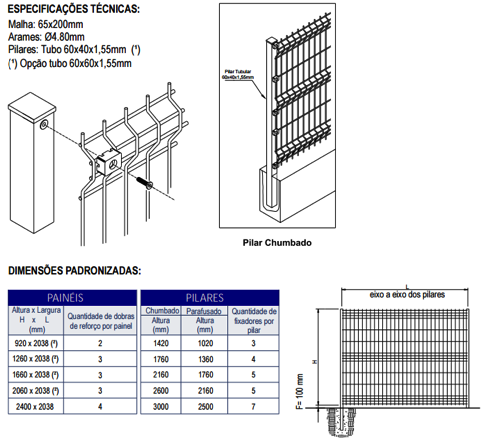
\includegraphics[keepaspectratio=true,scale=0.8]{figuras/EspecificacoesTecnicasCerca.png}
	\caption{Especifica\c{c}\~oes t\'ecnicas para a montagem da cerca}
	\small{Fonte: \cite{CatalogoCercamento}}
\end{figure}

O passo a passo a seguir mostra detalhadamente cada etapa do procedimento de instala\c{c}\~ao do gradil, que deve ser seguindo \`a risca para que n\~ao haja nem um tipo de problema no cercamento posteriormente \`a instala\c{c}\~ao da grade: 

\textbf{1$^{o}$ Passo: Funda\c{c}\~ao} \\ Primeiro deve-se delimitar o alinhamento e fazer a funda\c{c}\~ao de acordo com o tamanho do eixo do gradil escolhido com 200mm e profundidade de 500mm

\begin{figure}[h!]
	\centering
	\label{GradilEscolhido}
		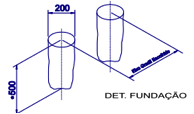
\includegraphics[keepaspectratio=true,scale=0.9]{figuras/GradilEscolhido.png}
	\caption{Passo 1, funda\c{c}\~ao para o gradil escolhido}
	\small{Fonte: \cite{CatalogoCercamento}}
\end{figure}

\textbf{2$^{o}$ Passo: Pr\'e montagem} \\ Neste segundo passo deve-se fazer a  pr\'e montagem dos pain\'eis e posteriormente posiciona-los em p\'e e apoia-los

\begin{figure}[h!]
	\centering
	\label{MontagemPaineisPilares}
		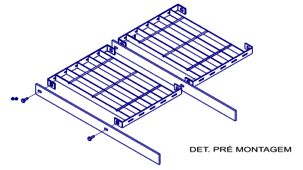
\includegraphics[keepaspectratio=true,scale=0.8]{figuras/MontagemPaineisPilares.png}
	\caption{Passo 2, montagem dos pain\'eis e pilares}
	\small{Fonte: \cite{CatalogoCercamento}}
\end{figure}

\textbf{3$^{o}$ Passo: Montagem sequencial} \\ Neste passo deve-se pegar os demais pain\'eis e ir montando seguindo o passo anterior(passo 2) e assim ate o termino da montagem

\begin{figure}[h!]
	\centering
	\label{MontagemSequencialPaineis}
		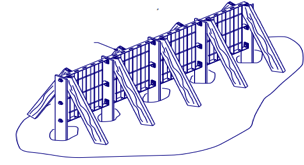
\includegraphics[keepaspectratio=true,scale=0.8]{figuras/MontagemSequencialPaineis.png}
	\caption{Passo 3, montagem sequencial de todos pain\'eis}
	\small{Fonte:  \cite{CatalogoCercamento}}
\end{figure}

\textbf{4$^{o}$ Passo: Aprumar e alinhar} \\ Nesta etapa deve-se estender as linhas superior e inferior entre o primeiro e o ultimo painel para alinhar o conjunto, ajustando as escoras para conservar o alinhamento

\textbf{5$^{o}$ Passo: Concretagem} \\ Neste \'ultimo passo deve-se concretar as bases da cerca e mante-las escoradas por no m\'inimo 24 horas

\begin{figure}[h!]
	\centering
	\label{ConcretagemBasesPilares}
		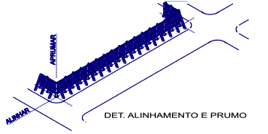
\includegraphics[keepaspectratio=true,scale=0.8]{figuras/ConcretagemBasesPilares.png}
	\caption{Passo 5, concretagem das bases dos pilares}
	\small{Fonte: \cite{CatalogoCercamento}}
\end{figure}

\subsection{Relat\'orio de Pain\'eis Solares}

\subsubsection{Objetivos}

Pesquisar empresas e produtos relacionados com o sistema de gera\c{c}\~ao de energia fotovoltaica, para a aplica\c{c}\~ao no Parque Vivencial e Urban\'istico do Gama e decidir por uma empresa, ou por requisitos para uma licita\c{c}\~ao.

\subsubsection{Comparativos das tecnologias dos sistemas fotovoltaicos}

Um sistema fotovoltaico \'e normalmente classificado em \textbf{Sistema Isolado}  (n\~ao conectado a rede el\'etrica da concession\'aria) ou \textbf{Sistema Conectado}  (conectado a rede el\'etrica da concession\'aria) e \'e usual mente constitu\'ido por:

 \begin{itemize}
        \item Painel fotovoltaico
	\item Regulador de Carga		(para sistemas isolados)
	\item Inversor
	\item Baterias	(para sistemas isolados)
\end{itemize}

Os sistemas existentes s\~ao os seguintes:

\begin{itemize}
        \item Sistemas isolados dom\'esticos (\textit{Off-grid domestic}): sistemas que fornecem energia el\'etrica para ilumina\c{c}\~ao, refrigera\c{c}\~ao e outras pequenas cargas em locais isolados. 
	\item Sistemas isolados n\~ao dom\'esticos (\textit{Off-grid non-domestic}): sistemas que fornecem energia el\'etrica a servi\c{c}os, tais como, telecomunica\c{c}\~oes, bombeamento de \'agua, frigor\'ificos m\'edicos, ajuda \`a navega\c{c}\~ao a\'erea e mar\'itima, esta\c{c}\~oes de recolha de dados meteorol\'ogicos.
	\item Sistemas distribu\'idos conectados \`a rede (\textit{Grid-connected distributed}): sistemas que fornecem energia el\'etrica a edif\'icios (comerciais ou industriais) ou outras cargas que tamb\'em est\~ao ligadas \`a rede, para onde a energia em excesso \'e enviada. A pot\^encia t\'ipica para este tipo de aplica\c{c}\~oes varia entre 0,5 kW e 100 kW.
	\item Sistemas centralizados conectados \`a rede (\textit{Grid-connected centralized}): sistemas que fornecem exclusivamente energia el\'etrica \`a rede.
\end{itemize}

\subsubsection{Sistemas isolados}

Os sistemas isolados ou aut\^onomos para gera\c{c}\~ao de energia solar fotovoltaica s\~ao caracterizados por n\~ao se conectarem a rede el\'etrica. O sistema abastece diretamente os aparelhos que utilizar\~ao a energia e s\~ao geralmente constru\'idos com um prop\'osito, local e espec\'ifico. Esta solu\c{c}\~ao \'e muito utilizada em locais remotos, j\'a que muitas vezes \'e o modo mais econ\^omico e pr\'atico de se obter energia el\'etrica nestes locais. \\ Os sistemas isolados de gera\c{c}\~ao de energia solar fotovoltaica, de maneira simplificada, s\~ao compostos de quatro componentes:

 \begin{itemize}
        \item \textbf{Pain\'eis solares ou placas solares:} s\~ao eles que geram a energia el\'etrica que abastece as baterias. Tem a propriedade de transformar a radia\c{c}\~ao solar em corrente el\'etrica cont\'inua. Um sistema pode ter apenas um painel ou v\'arios pain\'eis interligados entre si.
	\item \textbf{Controladores de carga:} garantem o correto abastecimento das baterias evitando sobrecargas e aumentando sua vida \'util.
	\item \textbf{Inversores:} s\~ao o c\'erebro do sistema e tem a fun\c{c}\~ao de transformar corrente continua (CC) em corrente alternada (AC), e levar a tens\~ao, por exemplo, de 12V para 127V. Em alguns casos pode ser ligado a outro tipo de gerador ou \`a pr\'opria rede el\'etrica para abastecer as baterias.
	\item \textbf{Baterias:} s\~ao os reservat\'orios do sistema e armazenam a energia el\'etrica para ser utilizada nos momentos em que o sol n\~ao esteja presente e n\~ao haja outras fontes de energia.
\end{itemize}

\subsubsection{Sistemas conectados a rede}

Em aplica\c{c}\~oes ligadas \`a rede de energia el\'ectrica, o gerador fotovoltaico entrega \`a rede a m\'axima pot\^encia que, em cada instante, pode produzir. Entre o m\'odulo e a rede existem equipamentos de regula\c{c}\~ao e interface que otimizam as condi\c{c}\~oes de gera\c{c}\~ao e as adaptam \`as condi\c{c}\~oes de recep\c{c}\~ao impostas pela rede. Em termos esquem\'aticos, a situa\c{c}\~ao pode ser descrita como se ilustra na figura abaixo.

\begin{figure}[h!]
	\centering
	\label{SistemaFotovoltaico}
		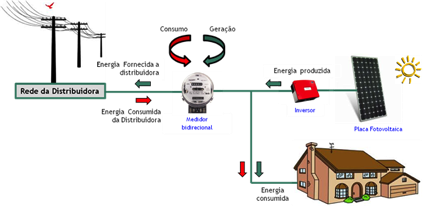
\includegraphics[keepaspectratio=true,scale=0.8]{figuras/SistemaFotovoltaico.png}
	\caption{Esquema de um sistema fotovoltaico ligado \`a rede}
	\small{Fonte:  \cite{Viridian}}
\end{figure}

Do ponto de vista dos componentes, um sistema fotovoltaico conectado \`a rede \'e similar ao sistema isolado com a diferen\c{c}a que o sistema conectado n\~ao necessita de baterias para armazenamento de energia.\\ 

Para a utiliza\c{c}\~ao no Parque Vivencial e Urban\'istico do Gama, n\~ao h\'a a necessidade de se instalar um sistema isolado, que \'e mais caro. Portanto o Sistema Conectado \`a rede \'e mais vi\'avel.

\subsubsection{An\'alise do Projeto}

A partir das plantas do projeto foi estimado um valor de consumo el\'etrico, usando uma simula\c{c}\~ao, para as seguintes edifica\c{c}\~oes:

 \begin{itemize}
        \item Sede Administrativa
	\item Guaritas
	\item Quiosques
	\item Banheiros
\end{itemize}

\begin{itemize}
      \item Sede Administrativa
             \begin{itemize}
                       \item \'Area \'util para placa solar	=	59,032 m$^{2}$ 
                       \item Consumo el\'etrico estimado	=	787,37 kWh 
	     \end{itemize}
\end{itemize}

\begin{figure}[h!]
	 \centering
	 \label{SistemaGeradorSede}
	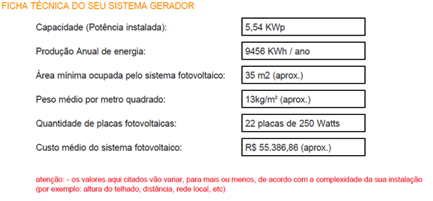
\includegraphics[keepaspectratio=true,scale=0.8]{figuras/SistemaGeradorSede.png}
	\caption{Ficha t\'ecnica do sistema gerador da Sede Administrativa}
	\small{Fonte: \protected\cite{PortalSolar}}
\end{figure}

\begin{itemize}
         \item Banheiro (x2)
	           \begin{itemize}
                       \item \'Area \'util para placa solar	=	21,824 m$^{2}$ 
                       \item Consumo el\'etrico estimado	=	89,88 kWh 
                  \end{itemize}	 
\end{itemize}

\begin{figure}[h!]
	  \centering
	 \label{SistemaGeradorBanheiro}
	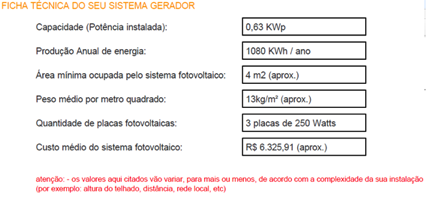
\includegraphics[keepaspectratio=true,scale=0.8]{figuras/SistemaGeradorBanheiro.png}
	\caption{Ficha t\'ecnica do sistema gerador do banheiro}
	\small{Fonte: \protected\cite{PortalSolar}}
\end{figure}

\begin{itemize}
         \item Guarita (x2)
	           \begin{itemize}
                       \item \'Area \'util para placa solar	=	8,41 m$^{2}$ 
                       \item Consumo el\'etrico estimado	=	77,62 kWh  
                  \end{itemize}	
\end{itemize} 

 \begin{figure}[h!]
	\centering
	\label{SistemaGeradorGuarita}
	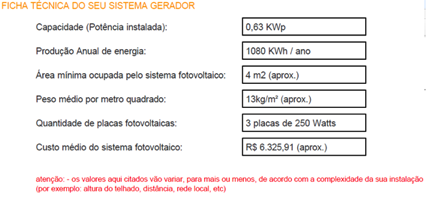
\includegraphics[keepaspectratio=true,scale=0.8]{figuras/SistemaGeradorBanheiro.png}
	\caption{Ficha t\'ecnica do sistema gerador da Guarita}
	\small{Fonte: \protected\cite{PortalSolar}}
\end{figure}

\begin{itemize}
         \item Quiosque (x2)
	           \begin{itemize}
                       \item \'Area \'util para placa solar	=	25 m$^{2}$ 
                       \item Consumo el\'etrico estimado	=	466,10 kWh      
                  \end{itemize}	 
\end{itemize}

\begin{figure}[h!]
	 \centering
	\label{SistemaGeradorQuiosque}
	 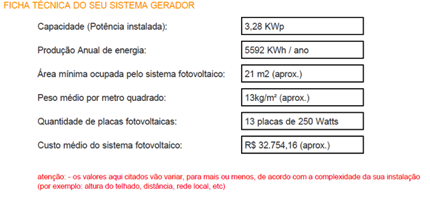
\includegraphics[keepaspectratio=true,scale=0.8]{figuras/SistemaGeradorQuiosque.png}
	 \caption{Ficha t\'ecnica do sistema gerador do Quiosque}
	\small{Fonte: \protected\cite{PortalSolar}}
\end{figure}

Total

 \begin{itemize}
        \item \'Area \'util para placa solar	=	169,5 m$^{2}$ 
        \item \'Area necess\'aria	=	93 m$^{2}$ 
        \item Consumo el\'etrico estimado	=	2054,57 kWh
	\item Quantidade de placas necess\'arias	=	60 (de 250 W)
	\item Custo do sistema + instala\c{c}\~ao	=	144.511,92 reais
\end{itemize}

\subsection{Projeto de ilumina\c{c}\~ao}

\subsubsection{Defini\c{c}\~oes de Termos Luminot\'ecnicos}

Para uma maior compreens\~ao do projeto ser\'a abordado alguns termos luminot\'ecnicos e el\'etricos necess\'arios para a compreens\~ao das demais se\c{c}\~oes. De acordo com o manual de ilumina\c{c}\~ao p\'ublica da Copel, temos:

 \begin{itemize}
        \item Fluxo Luminoso - O fluxo luminoso pode ser entendido como a quantidade de energia radiante em todas as dire\c{c}\~oes, emitida por unidade de tempo, e avaliada de acordo com a sensa\c{c}\~ao luminosa produzida. A unidade de medida \'e o l\'umen (lm).
	\item Efici\^encia Luminosa - A efici\^encia luminosa \'e a rela\c{c}\~ao entre o fluxo luminoso emitido pela pot\^encia el\'etrica absorvida, sendo a unidade de medida o l\'umen por Watt (lm/W). Este conceito \'e utilizado para comparar a diferentes fontes luminosas.
	\item Iluminamento ou ilumin\^ancia - ilumin\^ancia \'e a densidade de fluxo luminoso recebido por uma superf\'icie. Por defini\c{c}\~ao a unidade de medida \'e o l\'umen por metro ao quadrado (lm/m$^{2}$), que pode ser denominada tamb\'em de lux. A verifica\c{c}\~ao deste par\^ametro \'e fundamental para comprovar a qualidade da ilumina\c{c}\~ao de um determinado local.
	\item Fator de uniformidade - O fator de uniformidade \'e uma rela\c{c}\~ao entre a ilumin\^ancia m\'inima e a m\'edia de uma determinada \'area. Resulta em um valor adimensional variando entre zero e a unidade, que indica como est\'a a distribui\c{c}\~ao da luminosidade na superf\'icie aferida. Umin = Emed/Emin (Manual de Ilumina\c{c}\~ao P\'ublica fevereiro de 2012 SED/DNGO/VNOT P\'agina 4)
	\item Temperatura de cor - Este par\^ametro n\~ao est\'a relacionado com o calor emitido por uma l\^ampada, mas pela sensa\c{c}\~ao de conforto que a mesma proporciona em um determinado ambiente. Quanto mais alto for o valor da temperatura de cor, mais branca ser\'a a luz emitida, denominada comumente de ?luz fria? e que \'e utilizada, por exemplo, em ambientes de trabalho, pois induz maior atividade ao ser humano. No entanto, caso seja baixa a temperatura de cor, a luz ser\'a mais amarelada, proporcionando uma maior sensa\c{c}\~ao de conforto e relaxamento, chamada popularmente de ?luz quente?, utilizada preferencialmente em salas de estar ou quartos. As fontes luminosas artificiais podem variar entre 2000K (muito quente) at\'e mais de 10000K (muito fria).
	\item \'Indice de reprodu\c{c}\~ao de cor - O \'indice de reprodu\c{c}\~ao de cor (IRC) de uma fonte luminosa \'e a medida de cor real de uma superf\'icie e sua apar\^encia a ser iluminada pela fonte artificial. Uma fonte com IRC 100\% \'e a que apresenta as cores de um objeto com a m\'axima fidelidade. Na Figura abaixo, \'e apresentado o mesmo local sob as mesmas condi\c{c}\~oes, por\'em iluminado com fontes luminosas diferentes. \`a esquerda a ilumina\c{c}\~ao \'e feita por LED?s (light emitting diode ou diodo emissor de luz) de alto IRC, e \`a direita com l\^ampadas a vapor de s\'odio em alta press\~ao com baixo IRC. Nota-se que na segunda situa\c{c}\~ao a defini\c{c}\~ao das cores \'e prejudicada
\end{itemize}

\begin{figure}[h!]
	 \centering
	\label{ComparativoDuasFontesLuminosas}
	 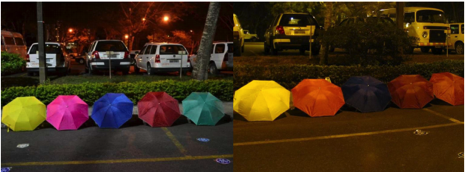
\includegraphics[keepaspectratio=true,scale=0.8]{figuras/ComparativoDuasFontesLuminosas.png}
	 \caption{Comparativo entre duas fontes luminosas com diferentes IRC?s}
	\small{Fonte: Copel e GE ? (General Eletric) - (Manual de Ilumina\c{c}\~ao P\'ublica fevereiro de 2012 SED/DNGO/VNOT P\'agina 5)}
\end{figure}

\begin{itemize}
        \item Vida mediana- Tempo ap\'os o qual 50\% das l\^ampadas de uma determinada amostragem, submetidas a um ensaio de vida, deixam de funcionar.
	\item Distor\c{c}\~ao harm\^onica total - Entende-se por distor\c{c}\~ao harm\^onica total (THD ? Total Harmonic Distortion), a rela\c{c}\~ao entre a soma dos valores eficazes de todas as componentes harm\^onicas de uma determinada forma de onda pelo valor eficaz de sua componente fundamental, expresso normalmente em termos percentuais. Para este manual, define-se THDi como a distor\c{c}\~ao harm\^onica da corrente absorvida por uma carga n\~ao linear, em geral equipamentos eletroeletr\^onicos, em rela\c{c}\~ao \`a onda senoidal pura com frequ\^encia de 60Hz, fornecida pela concession\'aria. Com relativa intensidade, uma corrente com elevado THDi pode provocar distor\c{c}\~oes nas formas de onda da corrente e tens\~ao do sistema el\'etrico, reduzindo a qualidade da energia entregue e prejudicando o funcionamento de outros equipamentos conectados \`a mesma rede. \cite{CopelParana}(Manual de Ilumina\c{c}\~ao P\'ublica fevereiro de 2012 SED/DNGO/VNOT P\'agina 6)
\end{itemize}

\begin{figure}[h!]
	 \centering
	\label{FormulaTHDI}
	 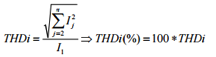
\includegraphics[keepaspectratio=true,scale=0.8]{figuras/FormulaTHDI.png}
	 \caption{F\'ormula THDi}
\end{figure}

Em que: \\ I$_{j}$ \'e o valor eficaz da componente harm\^onica da corrente absorvida pela carga ?e?. \\ I$_{1}$ \'e a componente fundamental da corrente, com frequ\^encia de 60Hz. \\ THDi(\%) \'e a distor\c{c}\~ao harm\^onica total da corrente expressa em valores percentuais.

\begin{itemize}
        \item Fator de Pot\^encia - O fator de pot\^encia \'e definido pela raz\~ao entre as pot\^encias ativa (P) e aparente (S) de um circuito, resultando em um n\'umero adimensional entre zero e um. Quanto mais pr\'oximo da unidade for o fator de pot\^encia, indica que a energia est\'a sendo consumida de forma mais eficiente, visto que apenas a pot\^encia ativa realiza trabalho efetivamente. No entanto, quanto mais pr\'oximo a zero indica que a maior parte da energia consumida \'e reativa, necess\'aria para o funcionamento de elementos armazenadores de energia, como indutores e capacitores, mas que deve ser compensada, pois gera perdas e diversas perturba\c{c}\~oes no sistema el\'etrico. A equa\c{c}\~ao completa para o c\'alculo do fator de pot\^encia \'e dada por:
\end{itemize}

\begin{figure}[h!]
	 \centering
	\label{FormulaFP}
	 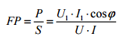
\includegraphics[keepaspectratio=true,scale=0.8]{figuras/FormulaFP.png}
	 \caption{F\'ormula FP}
\end{figure}

Onde: U$_{1}$ e I$_{1}$ s\~ao os valores eficazes das componentes fundamentais da tens\~ao e corrente, respectivamente, de um circuito \\
U e I s\~ao os valores eficazes totais da tens\~ao e corrente, respectivamente, calculados da seguinte forma:

\begin{figure}[h!]
	 \centering
	\label{FormulaX}
	 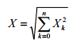
\includegraphics[keepaspectratio=true,scale=0.8]{figuras/FormulaX.png}
	 \caption{F\'ormula X}
\end{figure}

Em que: X$_{k}$ \'e o valor eficaz da componente harm\^onica que comp\~oe a forma de onda.
cos $\phi$ \'e o co-seno do \^angulo $\phi$ de desfasamento entre a corrente e a tens\~ao. (Manual de Ilumina\c{c}\~ao P\'ublica fevereiro de 2012 SED/DNGO/VNOT P\'agina 7) \\ Na maioria dos casos, as tens\~oes e correntes do sistema el\'etrico podem ser consideradas senoidais puras, logo seus valores eficazes totais s\~ao iguais aos de suas componentes fundamentais. Assim a equa\c{c}\~ao para o c\'alculo do fator de pot\^encia se resume ao co-seno do \^angulo $\phi$: FP = cos$\phi$ \\ No entanto, h\'a situa\c{c}\~oes no sistema el\'etrico em que as tens\~oes e correntes n\~ao s\~ao senoidais puras. Para estes casos a equa\c{c}\~ao geral para o c\'alculo do fator de pot\^encia deve ser utilizada. Para o c\'alculo do fator de pot\^encia dos equipamentos abrangidos por este manual, deve-se utilizar a equa\c{c}\~ao apresentada na sequ\^encia, que \'e resultado da inser\c{c}\~ao do conceito da total distor\c{c}\~ao harm\^onica da corrente apresentada na Distor\c{c}\~ao Harm\^onica Total. Na equa\c{c}\~ao geral, desprezando as poss\'iveis distor\c{c}\~oes na forma de onda da tens\~ao. Observa-se que, caso a corrente absorvida pela carga seja senoidal pura, o valor de THDi ser\'a nulo, e o resultado da equa\c{c}\~ao ser\'a apenas o co-seno do \^angulo de desfasamento entre a tens\~ao e a corrente.

\begin{figure}[h!]
	 \centering
	\label{FormulaFP2}
	 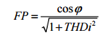
\includegraphics[keepaspectratio=true,scale=0.8]{figuras/FormulaFP2.png}
	 \caption{F\'ormula FP utilizando THDi}
\end{figure}

\subsubsection{Projeto de Ilumina\c{c}\~ao P\'ublica de \'Areas para Pedestres}

A ilumina\c{c}\~ao p\'ublica nas \'areas utilizadas predominantemente por pedestres deve prover seguran\c{c}a, conforto e a capacidade de reconhecer os eventos ao seu redor a uma dist\^ancia razo\'avel. \cite{CopelParana}(Projetos de Ilumina\c{c}\~ao P\'ublica novembro de 2012 Cemig P\'agina 5.1)

\subsubsection{Ilumina\c{c}\~ao de Pra\c{c}as e Parques}

Nas cidades, as pra\c{c}as e parques contribuem n\~ao s\'o para o embelezamento, mas tamb\'em promovem o lazer, recrea\c{c}\~ao e o conv\'ivio entre as pessoas. Dessa forma, uma aten\c{c}\~ao especial deve ser dada na elabora\c{c}\~ao dos projetos de ilumina\c{c}\~ao destes espa\c{c}os p\'ublicos, no sentido de torn\'a-los seguros e convidativos \`a comunidade. Contudo, a ilumina\c{c}\~ao \'e apenas um dos muitos componentes respons\'aveis pela melhoria do ambiente urbano. Sempre que necess\'ario, deve-se promover uma reforma nas condi\c{c}\~oes desses espa\c{c}os p\'ublicos.\cite{CemigMinas} \\ Algumas pra\c{c}as ou parques, em fun\c{c}\~ao de sua concep\c{c}\~ao arquitet\^onica, apresentam \'areas distintas de utiliza\c{c}\~ao como jardins, brinquedos, jogos de mesa, quadras, etc. Nestes casos, podem ser aplicados crit\'erios de projetos diferenciados para cada espa\c{c}o. Efeitos atrativos podem ser criados pelo uso de l\^ampadas com temperatura de cor diferente. Por exemplo, se utilizarmos l\^ampadas VS para a ilumina\c{c}\~ao do entorno, o interior da pra\c{c}a pode ser iluminada com l\^ampadas VMT.\cite{CemigMinas} \\ A ilumina\c{c}\~ao de escadas e rampas para acesso dos pedestres deve ser ponto de aten\c{c}\~ao e considerados na loca\c{c}\~ao dos postes de forma que estas mudan\c{c}as de n\'ivel sejam bem vis\'iveis. Est\'atuas, \'arvores, coretos e outros pontos de interesse especial, podem ser individualmente iluminados. Postes com altura de montagem superior a 5 metros somente devem ser instalados em pra\c{c}as e cal\c{c}ad\~oes onde \'e poss\'ivel o acesso dos ve\'iculos de manuten\c{c}\~ao. Esta restri\c{c}\~ao vale tamb\'em para os espa\c{c}os onde o piso n\~ao estiver adequado ao peso destes ve\'iculos. Se uma pra\c{c}a possuir pequenas dimens\~oes, a melhoria da ilumina\c{c}\~ao das vias do entorno pode evitar a instala\c{c}\~ao de um projeto espec\'ifico. Nos cal\c{c}ad\~oes, a disposi\c{c}\~ao da ilumina\c{c}\~ao n\~ao deve obstruir o acesso dos ve\'iculos de emerg\^encia ou de manuten\c{c}\~ao.\cite{CemigMinas} 

\subsubsection{N\'iveis de iilumin\^ancia e uniformidade}

A ilumina\c{c}\~ao destes espa\c{c}os deve permitir no m\'inimo um reconhecimento m\'utuo, al\'em de proporcionar informa\c{c}\~ao visual suficiente a respeito das pessoas e suas inten\c{c}\~oes a uma dist\^ancia segura. Segundo estudos realizados, a dist\^ancia m\'inima necess\'aria para uma pessoa reconhecer qualquer sinal de hostilidade e tomar as a\c{c}\~oes evasivas apropriadas \'e de 4 metros. A esta dist\^ancia, o n\'ivel de ilumin\^ancia m\'edio m\'inimo necess\'ario para reconhecimento facial \'e de 5 lux. De toda forma, sobre a superf\'icie n\~ao deve haver valor inferior a 1 lux. Considerando a necessidade de identifica\c{c}\~ao de obst\'aculos na superf\'icie da via e a velocidade com que as pessoas ou eventualmente ciclistas trafegam, o fator de uniformidade (U) n\~ao deve ser inferior a 0,25. A Tabela 1 apresenta as recomenda\c{c}\~oes para o n\'ivel de ilumin\^ancia m\'edia e informa o valor m\'inimo para o fator de uniformidade para cada classe de ilumina\c{c}\~ao de pedestres.\cite{CemigMinas}

\subsubsection{Ciclovia e ciclofaixa}

Considerando a import\^ancia crescente das bicicletas como meio de transporte nas cidades, a ilumina\c{c}\~ao das ciclovias contribui para a redu\c{c}\~ao dos acidentes o que \'e particularmente importante quando existem cruzamentos com vias de tr\^ansito de ve\'iculos automotores. Os principais requisitos de visibilidade a serem fornecidos pela ilumina\c{c}\~ao s\~ao:

\begin{itemize}
        \item As altera\c{c}\~oes no trajeto e os limites da ciclovia e ciclofaixa 
        \item A presen\c{c}a de obst\'aculos fixos na superf\'icie, tais como mobili\'ario urbano, \'arvores, etc
	\item A visualiza\c{c}\~ao de buracos e rachaduras na superf\'icie da pista
	\item A posi\c{c}\~ao e a velocidade dos usu\'arios da ciclovia
	\item A exist\^encia de cruzamentos com as vias que conduzem outro tipo de tr\'afego
\end{itemize}

As lumin\'arias utilizadas devem ser instaladas com espa\c{c}amentos m\'inimos de 3,5 vezes a altura de montagem. Para a maioria das ciclovias e ciclofaixas, os requisitos para a escolha da fonte de luz devem considerar os crit\'erios utilizados para a ilumina\c{c}\~ao das demais vias urbanas como vida mediana, rendimento. Contudo, pode ser necess\'ario utilizar uma l\^ampada de cor diferente da existente na via adjacente a fim de chamar a aten\c{c}\~ao dos motoristas quanto \`a exist\^encia da ciclovia ou ciclofaixa. A Tabela 1 apresenta as recomenda\c{c}\~oes para o n\'ivel de ilumin\^ancia m\'edia e informa o valor m\'inimo para o fator de uniformidade para ciclovias e ciclofaixas. Conforme a NBR 5101:1992 temos os limites fotom\'etricos para vias de trafego de pedestres segundo a tabela abaixo. \cite{CopelParana}(Manual de Ilumina\c{c}\~ao P\'ublica fevereiro de 2012 SED/DNGO/VNOT P\'agina 21)

\begin{table}[h!]
\caption{Limites fotom\'etricos para vias de tr\'afego motorizado e de pedestres} 
\begin{center}
\begin{tabular}{|p{8cm}|p{4cm}|p{4cm}|} \hline

Descri\c{c}\~ao da Via &E$_{m\'in}$ (lux) &U$_{m\'in}$ \\ \hline 

Vias de uso noturno intenso por pedestres (por exemplo, cal\c{c}ad\~oes, passeios de zonas comerciais) &20 &0,3 \\ \hline
Vias de grande tr\'afego noturno de pedestres (por exemplo, passeios de avenidas, pra\c{c}as, \'areas de lazer) &10 &0,25 \\ \hline
Vias de uso noturno moderado por pedestres (por exemplo, passeios, acostamentos) &5 &0,2 \\ \hline
Vias de pouco uso por pedestres (por exemplo, passeios de bairros residenciais) &3 &0,2 \\ \hline
Circuito da ciclovia ou ciclofaixa &5 &0,3 \\ \hline
Cruzamento de vias com trafego motorizado &10 &0,3 \\ \hline

 \end{tabular}
\end{center}
\end{table}

\subsubsection{\'Areas de Ilumina\c{c}\~ao}

De acordo com os padr\~oes de ilumina\c{c}\~ao p\'ublica estabelecidos pelas normas brasileiras, para manter o n\'ivel de m\'inimo de ilumina\c{c}\~ao ou ilumin\^ancia, obteve-se o seguinte padr\~ao de posicionamento dos poste de acordo com a figura abaixo:

\begin{figure}[h!]
	 \centering
	\label{PosicionamentoPostes}
	 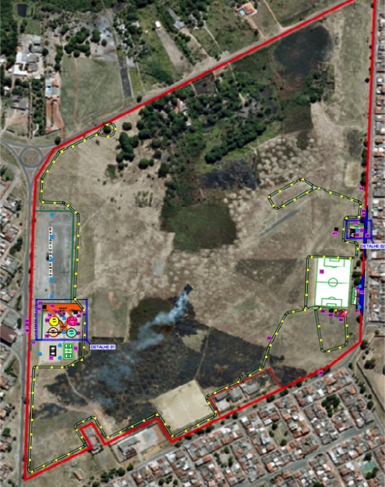
\includegraphics[keepaspectratio=true,scale=0.8]{figuras/PosicionamentoPostes.png}
	 \caption{Padr\~ao de posicionamento dos postes}
\end{figure}

Os pontos amarelos que est\~ao situados na ciclovia s\~ao os postes do modelo PTS 305/315 que distam aproximadamente 27 metros entre si, totalizando 103 postes ao longo de toda a ciclovia. Segue na  figura 2 abaixo as especifica\c{c}\~oes t\'ecnicas desse modelo:

\begin{figure}[H]
	 \centering
	\label{PTS305}
	 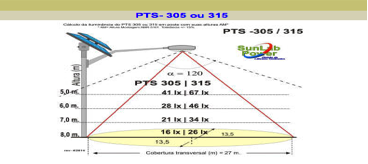
\includegraphics[keepaspectratio=true,scale=0.8]{figuras/PTS305.png}
	 \caption{Especifica\c{c}\~oes t\'ecnicas poste PTS - 305/315}
	 \small{Fonte: \cite{SUNLABPTS}}
\end{figure}

J\'a os pontos azuis que est\~ao situados nas \'areas de conviv\^encia social, s\~ao os postes do modelo PTS 405/410. Na \'area designada a um dos estacionamentos foram alocados 5 postes que distam entre si aproximadamente 30 metros, e no restante das \'areas de conviv\^encia social foram alocados postes de acordo com a necessidade, totalizando 13 postes desse modelo. Segue na figura 3 abaixo as especifica\c{c}\~oes t\'ecnicas desse modelo:

\begin{figure}[H]
	 \centering
	\label{PTS405}
	 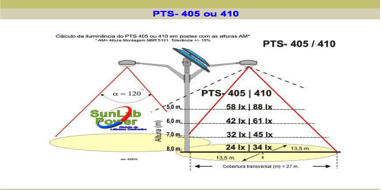
\includegraphics[keepaspectratio=true,scale=0.8]{figuras/PTS405.png}
	 \caption{Especifica\c{c}\~oes t\'ecnicas poste PTS - 405/410}
	 \small{Fonte: \cite{SUNLABPTS}}
\end{figure}

É importante atentar que o futuro campo de futebol a direita da imagem j\'a \'e iluminado, n\~ao sendo vi\'avel sua remo\c{c}\~ao, j\'a que os mesmos s\~ao espec\'ificos para campos e \'areas grandes que necessitam de bastante ilumina\c{c}\~ao, por\'em a esquerda no estacionamento, haver\'a a trocas dos postes existentes para os escolhidos neste ponto de controle, a substitui\c{c}\~ao dos mesmos acarretar\'a em uma economia de energia a longo prazo e o desvinculamento com a rede da CEB, padronizando assim a sua manuten\c{c}\~ao. \\ A tabela abaixo mostra os padr\~oes de luminot\'ecnicos dos postes avaliados e dos postes dos respectivos PTS - 305/315 e PTS - 405/10 que ser\~ao usados na revitaliza\c{c}\~ao do parque, os dois modelos escolhidos foram os que melhor se enquadraram nos padr\~oes de ilumina\c{c}\~ao segundo os manuais de ilumina\c{c}\~ao da companhias energ\'eticas dos estados da federa\c{c}\~ao:

\begin{figure}[H]
	 \centering
	\label{TabelaModelosPoste}
	 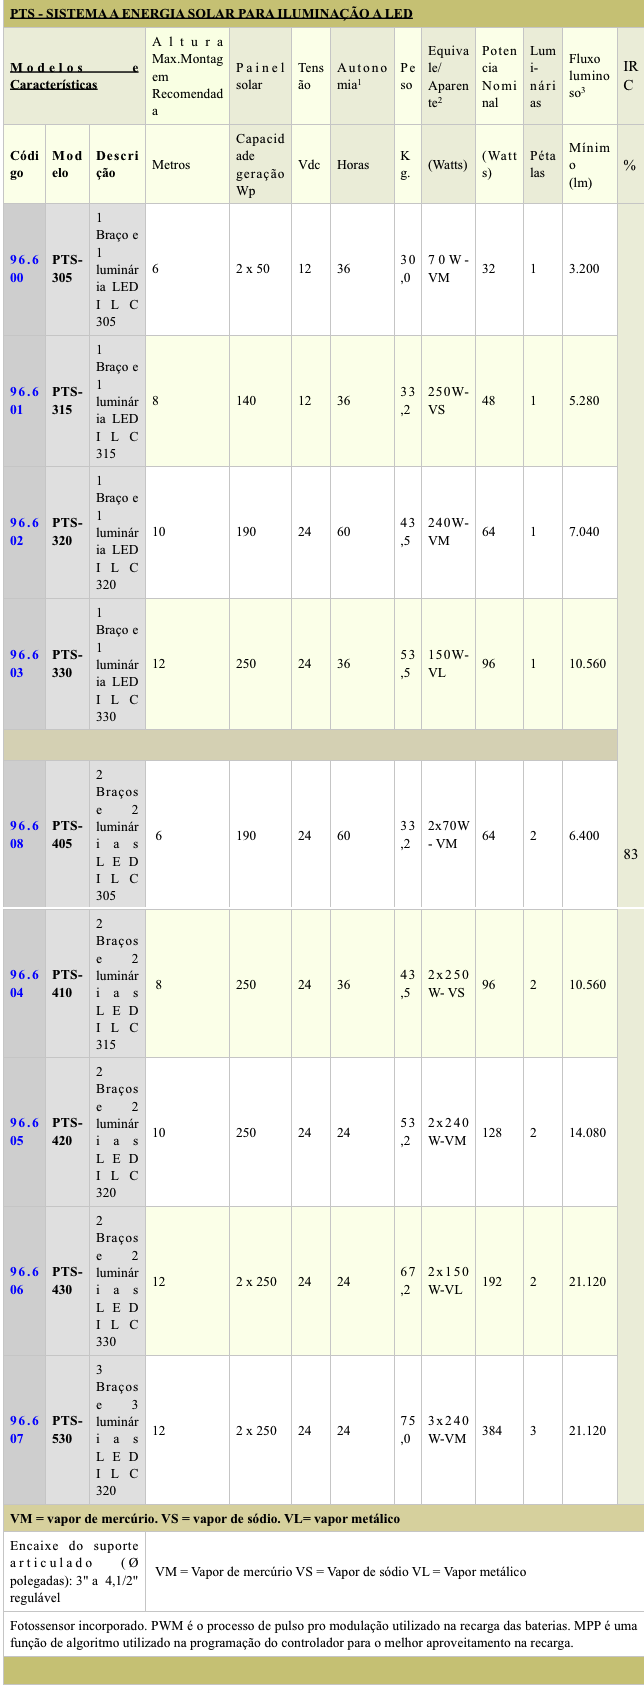
\includegraphics[keepaspectratio=true,scale=0.2]{figuras/TabelaModelosPoste.png}
	 \caption{Modelos de postes da linha PTS}
\end{figure}

\subsection{Interação social e atratividade do parque}

	A partir da problemática apresentada, a falta de atratividade do parque, o grupo de Interação Social definiu a orientação das soluções no sentido mais material, ou seja, no sentido de dar a estrutura necessária para que a futura administração do parque possa promover eventos e atividades educacionais com recursos tecnológicos.

	Fomentar a edução de jovens e crianças, promover atividades físicas à toda população próxima ao parque (desde jovens até o público idoso) foram as motivações que impulsionaram o grupo a pensar em soluções práticas, de custo acessível e disponível gratuitamente a toda a população do Gama.

	Sendo assim, todas as soluções estão integradas e promovendo a interação da comunidade afim de tornar as atividades de lazer contínuas e bem definidas.
	
	Primeiramente identificou-se a necessidade de um espaço para eventos e realizações de atividades recreativas como por exemplo:

\begin{itemize}
	\item Aulas de ginástica para jovens e idosos;
	\item Cinema comunitário e eventos de promoção ao lazer e cultura;
	\item Aulas temáticas para crianças e jovens, incentivando conhecimentos ambientais, regionais e que promovam os cursos da Faculdade UnB Gama (FGA) por exemplo;
	\item Eventos comunitários como festas comemorativas, assembléias de moradores, reuniões de grupos sociais e filantrópicos, entre outras utilidades. Esses eventos poderiam ser agendados gratuitamente na administração do parque;
\end{itemize}

	Todo esse ambiente social e de interação entre a comunidade do parque estaria reunido em um aplicativo para smartphones e tablets, onde os frequentadores do parque interagiriam com o ambiente com as pessoas que o frequentam, obteriam informações relevantes sobre o parque, sua construção, ambiente e curiosidades, bem como informações sobre eventos e sobre os outros frequentadores.

	Sendo um incentivo ao uso da tecnologia, o parque do gama atende a todas as preocupações dos usuários, portanto o parque contará com tomadas e carregadores de celular acessíveis ao público, nos locais de vivencia social.

	Haja vista toda essa gama de possibilidades de boas soluções para o parque, o grupo procurou adequar o projeto inicial, que já esta em implementação pela administração do Gama, às novas necessidades tecnológicas verificadas.

\subsubsection{Espaço interativo e vivência}

	Após discussões e análises em busca de uma primazia para o parque do Gama, chegou-se a uma dedução no que se refere ao fascínio por parte da população ao parque: Criação de um espaço multimídia.
Os elementos que compõem o escopo para que essa atratividade seja atingida são; Aulas interativas para a população, que contará com sistemas de áudio e video de alta tecnologia, gerando assim uma experiência única de aprendizagem. Práticas de exercícios físicos para a população com um viés de sustentabilidade, que será alcançado com aulas de spinning em bicicletas que gerarão energia elétrica. E para complementar, também serão realizados espetáculos e solenidades com o auxilio das tecnologias já mencionadas.

	Para que essas atividades sejam realizadas, uma estrutura física deverá ser erguida em formato de tenda, que terá um tamanho de 2.000 $m^{2}$, as figuras 1.1 e 1.2 mostram uma perspectiva da futura instalação. Esse espaço será constituído por uma estrutura metálica e por uma cobertura em PVC. A estrutura será fabricada em tubos de metalon de aço carbono com pontos soldados eletricamente em MIG e intervalado por parafusos com porca auto-travante, essa estrutura ficará em uma área fixa do parque, e com os devidos cuidados informados pelo fabricante deve possuir uma vida útil extremamente longa.
A cobertura em PVC será vulcanizada com sistema de termo fixação eletrônica, evitando-se assim o uso de costuras. A cobertura será em vinil VINISET que será impermeável, resistente a rasgos, bloqueador solar para melhor sensação térmica, auto-extinguível (não se propaga fogo), anti-fungo e anti-oxidante. Um dos pontos negativos em relação a cobertura será a sua durabilidade, a qual devido as condições naturais do tempo, possuem sua vida útil em torno de cinco anos.

	A inclinação para a escolha desse tipo de estrutura e não para as estruturas convencionais, como as de alvenaria, se deve ao fato do projeto ter como foco, o baixo custo. A única estrutura feita em alvenaria e representada na figura 1.3, será o deposito dos equipamentos do espaço, pois estes possuem alto valor e requerem uma maior segurança para que não sejam furtados. A conclusão do projeto, segundo empresas especializadas no segmento, terá como intervalo de tempo 90 dias, dentro desse tempo contará a criação e aprovação do projeto por engenheiro responsável.
	
\begin{figure}[H]
	 \centering
	\label{Tenda Modelo Padrão}
	 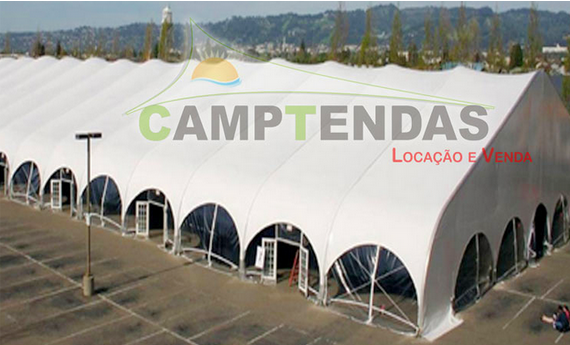
\includegraphics[keepaspectratio=true,scale=0.8]{figuras/TendaModeloGalpao.png}
	 \caption{Tenda Modelo Galpão}
	 \small{Fonte: camptendas.com.br}
\end{figure}

\begin{figure}[H]
	 \centering
	\label{Visão Interna Tenda}
	 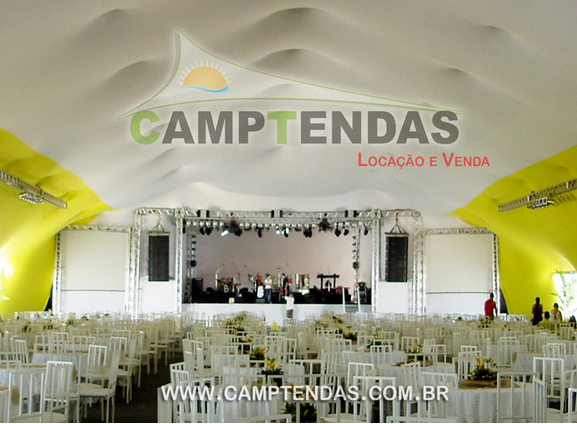
\includegraphics[keepaspectratio=true,scale=0.8]{figuras/VisaoInternaTenda.png}
	 \caption{Visão Interna da Tenda}
	 \small{Fonte: camptendas.com.br}
\end{figure}

\begin{figure}[H]
	 \centering
	\label{Deposito Dos Equipamentos}
	 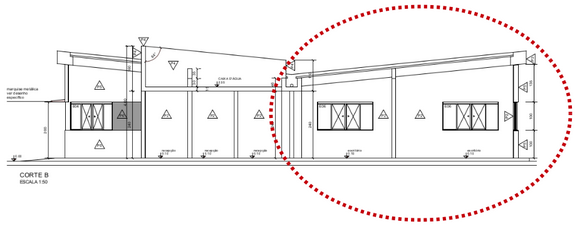
\includegraphics[keepaspectratio=true,scale=0.8]{figuras/DepositoDosEquipamentos.png}
	 \caption{Deposito dos equipamentos do espaço interativo}
	 \small{Fonte: Fornecida pela Administração Regional do Gama-DF}
\end{figure}

\subsubsection{Locais permitidos para construção no Parque Vivencial do Gama}

	Dentro do Parque do Gama existem nascentes que restringem qualquer construção em um raio de 50 (cinquenta) metros das mesmas, de acordo com a Lei Federal 4.771/65, alterada pela Lei 7.803/89 e a Medida Provisória nº 2.166-67, de 24 de agosto de 2001, “Consideram-se de preservação permanente, pelo efeito de Lei, as áreas situadas nas nascentes, ainda que intermitentes e nos chamados ‘olhos d’água’, qualquer que seja a situação topográfica, devendo ter um raio mínimo de 50 (cinquenta) metros de largura”. 

	A área imediatamente circundante à nascente, em um raio de 50 (cinquenta) metros, é só e exclusivamente uma área de preservação permanente. A restrição para se fazer uso dessa área existe para evitar que, com um cultivo, por exemplo, a nascente fique sujeita à erosão e que as atividades agrícolas de preparo do solo, adubação, plantio, cultivos, colheita e transporte dos produtos levem trabalhadores, máquinas e animais de tração para o local, contaminando física, biológica e quimicamente a água.

	A área adjacente à nascente deve ser toda cercada a fim de evitar o acesso de animais, pessoas, veículos, etc. Todas as medidas devem ser tomadas para favorecer seu isolamento, tais como proibir a pesca e a caça, evitando-se a contaminação do terreno ou diretamente da água por indivíduos inescrupulosos. Quando da realização de alguma obra ou serviço temporário, devem-se construir fossas secas a 30 (trinta) metros, no mínimo, mantendo-se uma vigilância constante para não haver poluição da área circundante à nascente.

	Pode-se localizar na imagem abaixo as nascentes no Parque Vivencial do Gama, de acordo com o texto contendo informações técnicas do parque cedido pela Administração Regional do Gama – RA II, e com isso ter o embasamento de áreas que são permitidas fazer qualquer construção ou alteração.
	
\begin{figure}[H]
	 \centering
	\label{Regiões das nascentes e vederedas}
	 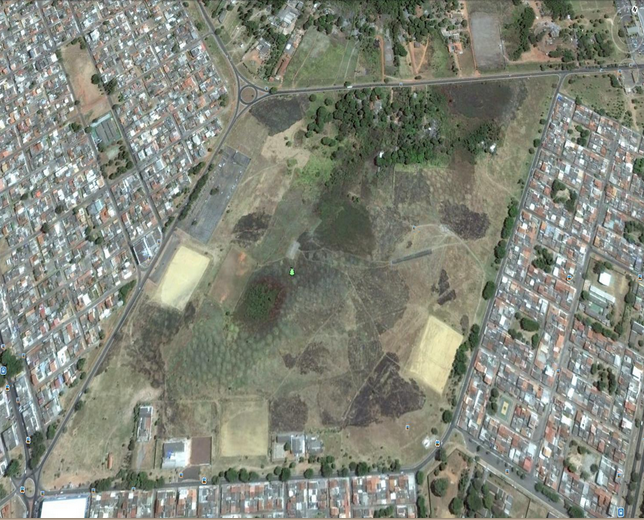
\includegraphics[keepaspectratio=true,scale=0.8]{figuras/RegioesDasNascentes.png}
	 \caption{Regiões acinzentadas são regiões de nascentes e veredas}
	 \small{Fonte: Google Earth}
\end{figure}

	No mapa abaixo está marcado onde será o espaço desenvolvido para os eventos no parque, o local fica próximo ao estacionamento. O motivo da escolha foi a facilidade e praticidade que as pessoas terão em encontrar e chegar ao local.

\begin{figure}[H]
	 \centering
	\label{Localização do espaço de eventos}
	 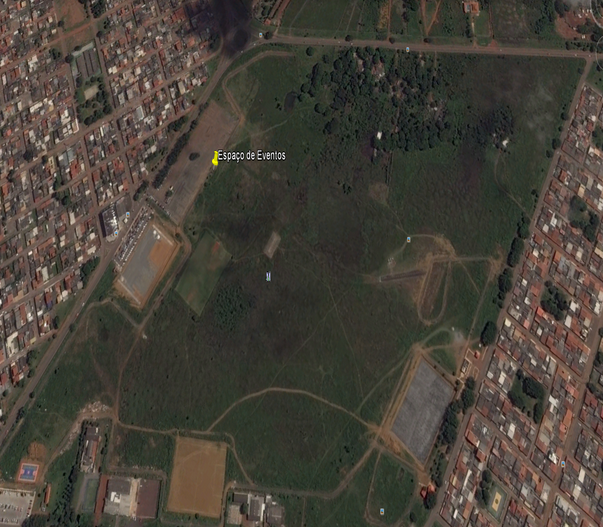
\includegraphics[keepaspectratio=true,scale=0.8]{figuras/LocalEspacoEvento.png}
	 \caption{Localização do Espaço de eventos}
	 \small{Fonte: Google Earth}
\end{figure}

\subsubsection{Sistemas de aulas de ginástica com bicicletas ergométricas sustentável}

	A idéia deste projeto é gerar energia elétrica de uma forma limpa, segura e sustentável, a partir da transformação de energia mecânica cinética, utilizando bicicletas ergométricas, em energia elétrica, que ficarão localizadas dentro do espaço  interativo e serão utilizadas para aulas de spinning com a comunidade do Gama, utilizando os telões e o sistema de sonorização para fazer a interação da aula e motivar os moradores a frequentar as aulas.

	Com base em um projeto de cinema ao ar livre e festivais de música em Londres, surgiu a idéia de adaptar as bicicletas em geradores para que toda energia transformada, seja enviada a uma estação de energia para ser utilizada como alimento para grandes telões, equipamentos de som. A idéia é muito promissora e deve ser aceita pela comunidade frequentadora do parque. É uma maneira sustentável que conta com a ajuda da comunidade para ter um ótimo funcionamento.
	
	Esse sistema de cinema ao ar livre já é utilizado em Londres, com apenas 30 bicicletas e é possível que 1000 pessoas possam assistir a um filme com a energia gerada. Nosso projeto não será ao ar livre, mas contará com a mesma capacidade. Serão adaptadas 30 bicicletas, em dois tamanhos para facilitar sua utilização a todos os públicos, podendo ter um público máximo de até 1000 pessoas.
	
\begin{figure}[H]
	 \centering
	\label{Funcionamento do Telão por energia gerada por bicicletas}
	 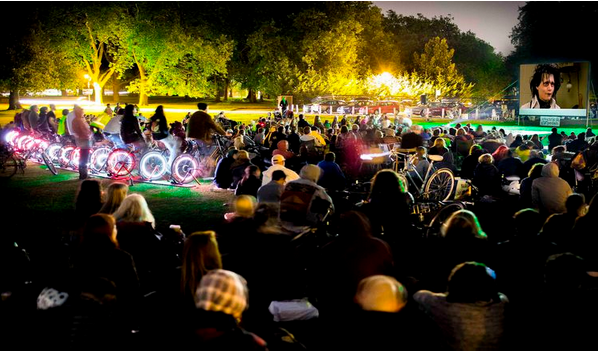
\includegraphics[keepaspectratio=true,scale=0.8]{figuras/TelaoFuncionamentoEnergiaBicicleta.png}
	 \caption{Telão em funcionamento com a energia gerada pelas bicicletas em Londres}
	 \small{Fonte: electricpedals.squarespace.com}
\end{figure}

\begin{figure}[H]
	 \centering
	\label{Evento realizado com as bicicletas}
	 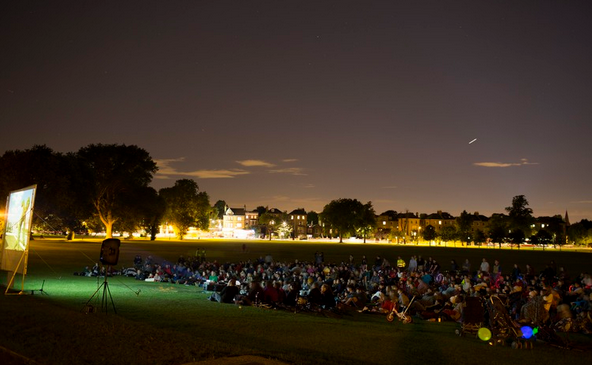
\includegraphics[keepaspectratio=true,scale=0.8]{figuras/TelaoFuncionamentoEnergiaBicicleta2.png}
	 \caption{Evento realizado com as bicicletas}
	 \small{Fonte: electricpedals.squarespace.com}
\end{figure}

\begin{figure}[H]
	 \centering
	\label{Festival de música}
	 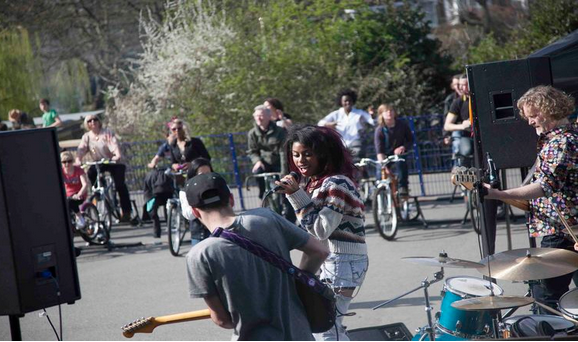
\includegraphics[keepaspectratio=true,scale=0.8]{figuras/TelaoFuncionamentoEnergiaBicicleta3.png}
	 \caption{Festival de música}
	 \small{Fonte: electricpedals.squarespace.com}
\end{figure}

\subsubsection{Produtos}

	Serão utilizadas 20 bicicletas de aro 26, com 18 marchas, e 10 bicicletas de aro 24, com preço aproximado de R\$230,00, com quadro de aço carbono, pesando aproximadamente 14kg, corrente fina, pedal de plástico e com garfo rígido. Serão adaptados em cada bicicletas pneus novos, estilo liso, para uma melhor eficiência. 
	
	Cada bicicleta seria acoplada a um suporte que estará ligado a um gerador, que será tracionado pelo pneu traseiro da bicicleta. O suporte e o gerador serão, baseados nos suporte e geradores da Eletric Pedals, que é um projeto feito em Peckham, Londres. Nesse projeto, utiliza-se bicicletas para gerar energia em pequenos eventos, para carregar notebooks, celulares, ligar telas e equipamentos de som onde as pessoas vão pedalando e com suas pedaladas geram energia para tal finalidade.
	
	Outra idéia que será usada como referencia é da Eletric Pedals, uma estação de energia (Power Station Quark) que administra eficientemente a energia produzida por até 30 pessoas utilizando seus geradores de Energia. Essa estação de energia não possui baterias, usa apenas ultra-capacitores para armazenar e reduzir a energia gerada antes, de fornecer uma segura fonte de alimentação AC 230 volts limpa.

\pagebreak
\begin{itemize}
	\item Bicycle Friction Generator: Gerador

	\begin{figure}[H]
	 \centering
	\label{Gerador bicicleta}
	 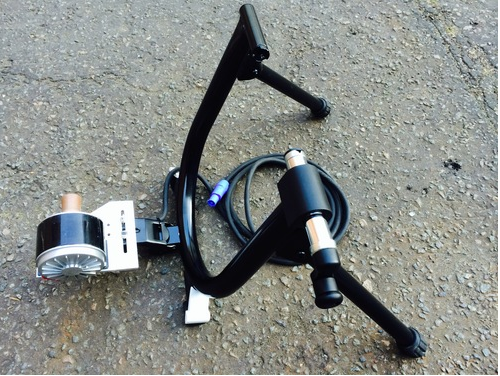
\includegraphics[keepaspectratio=true,scale=0.8]{figuras/bicycle.png}
	 \caption{Gerador no qual a bicicleta é acoplada, projetado para gerar eletricidade usando uma bicicleta padrão.}
	 \small{Fonte: electricpedals.squarespace.com}
	\end{figure}

	\begin{itemize}
	\item Características
	\end{itemize}

		Esse gerador, produz eletricidade regulamentada DC. Fornece um máximo de 400 watts, potência média durante um 	período de tempo geralmente em torno de 40-60 watts por pessoa. Possui 6-8m Heavy Duty cabo e conector rápido, bloqueio de diodo. 200 watts 24 volts motor de ímã permanente. Dobras para o armazenamento compacto e um peso de 7,5 Kg.
	
\begin{itemize}
	\item Aplicações
\end{itemize}	
	
	Escolas : Pode ser utilizado para aulas ao ar livre.
Aparelhos domésticos: Aparelhos de baixa potência, como laptops, música , iluminação e carregamento de celular. Mais aparelhos podem ser alimentados, quando combinados com a uma Mini Central Elétrica.
Banco de bateria: Pode ser usado para carregar uma bateria ou um banco de baterias.

\end{itemize}

\begin{itemize}
	\item Capacitor power station quark (Estação de enegia)
	
	Administra a energia produzida por até 30 pessoas que utilizam os geradores. Ele não tem baterias, utiliza alguns super eficiente ultra-capacitores para armazenar e suavizar a energia gerada antes de fornecer a uma fonte segura de AC230 volts limpos.
	\begin{itemize}
		\item Características
		Encerrados em pesados casos de voo, inversor de onda senoidal. Possui uma tensão de saída de 230 V AC ± 2\%. 2000 watts contínuo de potência de saída. Entrada máxima de 200 A para 30 pessoas. Além de possuir componentes reforçados é super eficiente.
	\end{itemize}
	
	\begin{itemize}
		\item Aplicações
		Cinema : Usado em conjunto com qualquer um gerador de energia, pode ser usada para alimentar um cinema ao ar livre para até 1000 pessoas.
Música: Pode em conjunto com um gerador alimentar um pequeno palco de música.
	\end{itemize}
	
	\begin{itemize}
		\item Especificações
		Possui uma saída do inversor de 2000 watts contìnua ( potência de pico de 4000 watts ), tem uma inversão máxima de 92\% de sua eficiência. 2000 Farad no ultra-capacitor. Uma gestão de tensão com base arduino. 2x251 A de fusíveis. Possui um ponto terra, 10 milímetros de um painel frontal em policarbonato transparente. Dimensões (LxPxA): 1,700 milímetros x 510 milímetros x 500 milímetro e um peso de 60 Kg.
	\end{itemize}
	
	\begin{figure}[H]
	 \centering
	\label{Estação de energia}
	 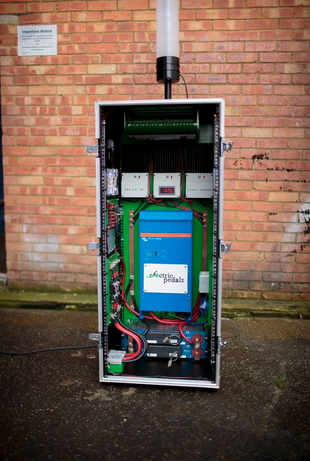
\includegraphics[keepaspectratio=true,scale=0.8]{figuras/capacitor.png}
	 \caption{Power Station Quark (Estação de Energia)}
	 \small{Fonte: electricpedals.squarespace.com}
	\end{figure}	
	
\end{itemize}

\pagebreak
\begin{itemize}
	\item Bus Board: Distribuidor
	
	\begin{figure}[H]
	 \centering
	\label{Bus Board: Distribuidor}
	 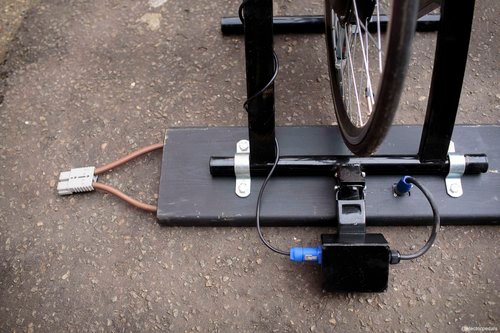
\includegraphics[keepaspectratio=true,scale=0.8]{interacao/11.png}
	 \caption{Gerador com bicicleta acoplada}
	 \small{Fonte: electricpedals.squarespace.com}
	\end{figure}
	
Os Distribuidores Bus Board são usados ​​para conectar-se rapidamente acima dos pares de qualquer um dos geradores de energia. Eles também fornecem uma plataforma estável para as pessoas a entrar e sair bicicletas e garantir que não há nenhum cabo solto.

	\begin{itemize}
	\item Características
	
	O design modular significa facilidade de configuração e arranjo.Pares de alumínio embutidos na base da placa, super base estável para a montagem segura de bicicletas. Perfil flush para fácil armazenamento, usa conectores bloqueáveis, extremamente robustos e confiáveis.				
	\end{itemize}	
			
	\begin{itemize}
	\item Vantagens
		Temos como vantagens uma configuração rápida, permitindo um grande número de geradores de fricção de bicicleta e geradores de cubo de bicicleta. Possue uma grande estabilidade, porque eles estão dispostos aos pares, cada pessoa fornece um lastro para a pessoa oposta. Os cabos são bem guardados para que as pessoas não venham tropeçar. Seu armazenamento é facilitado, pela falta de peças elevadas.	
	\end{itemize}		

	\begin{itemize}
	\item Especificações
		Suporte para duas unidades de geração de energia. Com um peso de 14,2 Kg. Um conector de bateria de 175 A ligados através de um cabo de cobre de 35 milímetro$s^{2}$. Com dimensões de L240cm x P21.5cm x H4.5cm
	\end{itemize}	

	\begin{itemize}
	\item Especificação de bicicleta para geração de energia
		O melhor tipo de bicicleta para a geração de energia é uma bicicleta estrada ou híbrido. Seus pneus traseiros lisos irá manter tanto ruído e fricção a um mínimo assegurando, e a melhor de transferência de energia.
	\end{itemize}
	
	\begin{itemize}
		\item Qualidades essenciais (Bicicleta para adulto)
		
		Engrenagens : Pelo menos cinco marchas para permitir o ajuste da geração de energia (sem fixie / bicicletas de velocidade única).
	
	\begin{figure}[H]
	 \centering
	\label{Engrenagem adequada}
	 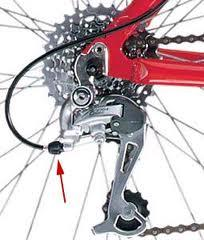
\includegraphics[keepaspectratio=true,scale=0.8]{interacao/12.png}
	 \caption{Engrenagem adequada}
	\end{figure}
	
	\begin{figure}[H]
	 \centering
	\label{Engrenagem inadequada}
	 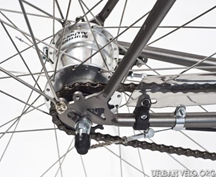
\includegraphics[keepaspectratio=true,scale=0.8]{interacao/13.png}
	 \caption{Engrenagem inadequada}
	\end{figure}		
	
	Pneus: Deve ter um pneu traseiro liso (ou, pelo menos, um padrão de piso consistente) . 
	
	\begin{figure}[H]
	 \centering
	\label{Pneu adequado}
	 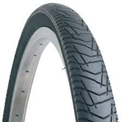
\includegraphics[keepaspectratio=true,scale=0.8]{interacao/14.png}
	 \caption{Pneu adequado}
	\end{figure}
	
	\begin{figure}[H]
	 \centering
	\label{Pneu inadequado}
	 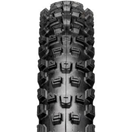
\includegraphics[keepaspectratio=true,scale=0.8]{interacao/15.png}
	 \caption{Pneu inadequado}
	\end{figure}
	
	\end{itemize}
	
	\begin{itemize}
	\item Qualidades opcionais
	
	Pequeno quadro : Para permitir que pessoas de todos os tamanhos possam andar de bicicleta. ( 14 "ou 15" ).

	Assento de liberação rápida : Para permitir o ajuste para ciclistas de diferentes tamanhos.
	
	Passo através do quadro : Para permitir a facilidade de entrar e sair 
	
	\begin{figure}[H]
	 \centering
	\label{Bicicleta adequada}
	 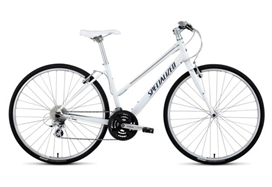
\includegraphics[keepaspectratio=true,scale=0.8]{interacao/16.png}
	 \caption{Bicicleta adequada}
	 \small{Fonte: electricpedals.squarespace.com}
	\end{figure}
		
	\end{itemize}
\end{itemize}

\subsubsection{Aplicativo}

	O avanço da tecnologia, tem tornado as pessoas cada vez mais próximas, independente da distância. Essa aproximação se dá, na maioria das vezes, por meio das redes sociais, sejam elas sites ou aplicativos. Devido a esse fato, pensou-se na ideia da criação de um aplicativo para o Parque Vivencial Urbano do Gama, o qual qualquer pessoa poderá baixá-lo em seu smartphone.
	
	A interface inicial do aplicativo possuirá links, como mapa do parque, agenda de eventos, texto descritivo e galeria de fotos do mesmo. Ao clicar no mapa o usuário terá acesso a uma lista de locais, como playgrounds, aparelhos para exercícios físicos, quiosques, banheiros, estacionamentos, nascentes e espaço de eventos. Para saber suas respectivas localizações e sobre o parque, basta clicar no local desejado e irá aparecer um outro mapa indicando sua localização e um link que levará à descrição. Clicando na agenda será aberta uma lista dos tipos de eventos, dentre eles estão música, teatro e exposições. Para saber as atrações e as datas o usuário deve clicar no evento desejado. Ele também encontrará a descrição do mesmo.

	Além de tudo as pessoas podem interagir entre si, por exemplo, comentar como está sendo um evento, comentar as fotos e sobre os locais onde elas estão naquele momento. Para isso é preciso fazer um rápido cadastro. Dessa forma, o parque se tornará mais atrativo, estimulando assim, as pessoas a frequentá-lo. 
Abaixo segue as imagens do aplicativo do Parque Ibirapuera, localizado em São Paulo, que serviu como exemplo para a criação do aplicativo para o Parque do Gama.

\begin{figure}[H]
	 \centering
	\label{Pagina inicial do aplicativo}
	 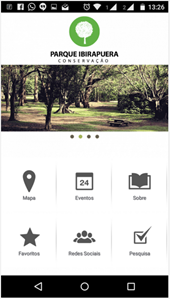
\includegraphics[keepaspectratio=true,scale=0.8]{interacao/17.png}
	 \caption{Pagina inicial.}
\end{figure}
	
\begin{figure}[H]
	 \centering
	\label{Seleção da opção para visualização do mapa}
	 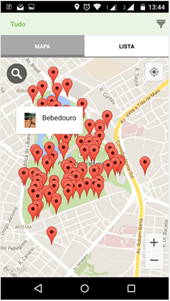
\includegraphics[keepaspectratio=true,scale=0.8]{interacao/18.png}
	 \caption{Seleção da opção para visualização do mapa.}
\end{figure}

\begin{figure}[H]
	 \centering
	\label{Seleção da opção para visualização da lista de locais}
	 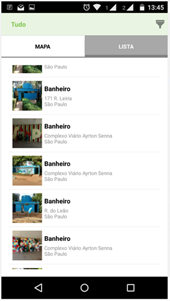
\includegraphics[keepaspectratio=true,scale=0.8]{interacao/19.png}
	 \caption{Seleção da opção para visualização da lista de locais.}
\end{figure}
	
\begin{figure}[H]
	 \centering
	\label{Seleção do local}
	 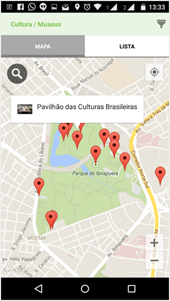
\includegraphics[keepaspectratio=true,scale=0.8]{interacao/20.png}
	 \caption{Seleção do local.}
\end{figure}

\begin{figure}[H]
	 \centering
	\label{Visualização de informações do local}
	 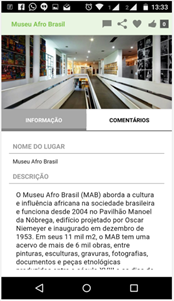
\includegraphics[keepaspectratio=true,scale=0.8]{interacao/21.png}
	 \caption{Visualização de informações do local.}
\end{figure}
\begin{figure}[H]
	 \centering
	\label{Seleção do local}
	 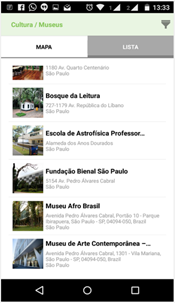
\includegraphics[keepaspectratio=true,scale=0.8]{interacao/22.png}
	 \caption{Seleção do local.}
\end{figure}
\begin{figure}[H]
	 \centering
	\label{Seleção para especificação do evento}
	 \includegraphics[keepaspectratio=true,scale=0.8]{interacao/23.png}
	 \caption{Seleção para especificação do evento.}
\end{figure}

\subsubsection{Ecoquiosques e postes com tomadas e acesso à WiFi}
	
	Atitudes ecológicas cada vez mais tem sido vistas como prioridade e assunto de extrema importância na atualidade em todo o mundo. Essas atitudes podem começar com pequenos gestos, com suas aplicações cada vez mais presentes no cotidiano das pessoas, inclusive em quiosques com aplicações sustentáveis.

	Como o  Parque Urbano do Gama já conta com um quiosque praticamente pronto em alvenaria. Um exemplo útil e prático se vê no desenvolvimento ou reaproveitamento de quiosques com visão sustentável, que apesar de poderem ser feitos em alvenaria possuem equipamentos de captação de luz solar, ou seja, placas fotovoltaicas que armazenam energia e contribuem para a iluminação e aquecimento do local,  tudo isso visando a economia de energia. Sua iluminação pode ser feita com luzes de LED, pois além de serem extremamente mais econômicas, têm maior durabilidade. Outro aspecto importante desses quiosques sustentáveis, são os sistemas de coleta e reutilização da água da chuva. Já que abaixo do telhado, que possui um declive, encontra-se um tanque de armazenamento de água da chuva coletada pela cobertura do local.
	
\begin{figure}[H]
	 \centering
	\label{Modelo de quiosque ecólogico}
	 \includegraphics[keepaspectratio=true,scale=0.8]{interacao/24.png}
	 \caption{Modelo de quiosque ecólogico.}
	 \small{Fonte: yankodesign.com/2011/04/08/ecokios/}
\end{figure}

\subsubsection{WiFi e Postes com USB no parque do Gama}
	
	É notório que a internet e os smartphones vieram pra ficar e a cada dia mais estão  presentes na vida das pessoas. O conceito de disponibilizar rede Wi-Fi de internet e postes com conectores USB para recarga de bateria de celulares no Parque Urbano do Gama, se deu justamente pra trazer atrativos a mais para a revitalização do mesmo, e consequentemente mais visitantes ao local. A população poderá utilizar a rede pra diversas atividades, com as principais sendo o lazer e os estudos.

	O conceito de Wi-fi livre surgiu através de um modelo já adotado em São Paulo – SP. Na cidade, a rede pertencente a praça Padre Aleixo Monteiro Mafra, conhecida como Praça do Forró, funciona 24 horas e comporta conexão simultânea de até 50 pessoas. Programas semelhantes ao Wi-fi Livre Parque Urbano Gama funcionam em cidades como Barcelona e Berlim. 	

	A velocidade da rede será de 512 Kbps por usuário, já que serão instalados três links de 25 Mpbs, o que permitirá atender até 150 usuários simultâneamente, algo que dependerá de 03 roteadores Mikrotik/RouterBoard modelo 1100. Para acessar a internet gratuita no Parque Urbano do Gama com o sistema em operação, o usuário deverá conectar seu smartphone, tablet ou nootbook na rede de Wi-fi do Parque, além de efetuar a autenticação por meio de um navegador de internet.
		
	Por outro lado, para iluminação do ambiente onde ficarão os quiosques ecológicos e onde a Wi-fi será estabelecida, serão implementados postes com técnologia de placas solares de 15 watts, que também possuirão conectores USB para que os visitantes possam utilizar mais esse recurso oferecido pelo Parque Urbano do Gama.
	
	Já esta outra idéia surgiu no Brooklyn, mais especificamente no Fort Green Park. São postes com suportes para apoio dos celulares por meio de conexão mini USB, iphone 4 e 5. As estruturas possuem três placas fotovoltaicas e baterias que armazenam a energia produzida. As baterias são  capazes de absorverem raios UV quando os dias estão nublados e podem ser carregas em até quatro horas nos dias de sol.

\begin{figure}[H]
	 \centering
	\label{Praça do forró em São Paulo}
	 \includegraphics[keepaspectratio=true,scale=0.8]{interacao/25.png}
	 \caption{Praça do Forro em São Paulo.}
	 \small{Fonte:wifilivre.sp.gov.br/}
\end{figure}

\begin{figure}[H]
	 \centering
	\label{Poste com placa fotovoltaíca}
	 \includegraphics[keepaspectratio=true,scale=0.8]{interacao/26.png}
	 \caption{Poste com placa fotovoltaíca no Brooklyn.}
	 \small{Fonte: jblog.jb.com.br/papodeambiente}
\end{figure}

\begin{figure}[H]
	 \centering
	\label{Carregador de celular USB em poste solar no Brooklyn}
	 \includegraphics[keepaspectratio=true,scale=0.8]{interacao/27.png}
	 \caption{Carregador de celular USB em poste solar no Brooklyn.}
	 \small{Fonte: jblog.jb.com.br/papodeambiente}
\end{figure}	

\subsection{Postes Solares}

\subsubsection{Estudo comparativo das tecnologias dos postes}
	O estudo realizado têm como propósito comparar tecnologias existentes no mercado utilizadas na iluminação pública utilizando placas solares, baterias e lampadas LED, para auxiliar na revitalização do Parque Urbano e Vivencial do Gama. Com base em tal pesquisa, realizou-se a escolha do poste, visando aspectos econômicos, financeiros e tecnológicos, além de fazer um balanço energético da energia produzida, e consumida pelos postes.

	O levantamento realizado mostrou que existem vários tipos de postes solares atualmente no mercado, os quais possuem  tecnologias diversas com aplicações distintas e em vários ambientes públicos.  Abaixo serão apresentados os estudos desses.

\begin{itemize}
	\item PIE - Produtor Independente de Energia
	
	Foi desenvolvido um poste autossustentável denominado PIE (Produtor Independente de Energia), no Ceará, pelo engenheiro mecânico e dono da Gram-Eollic Fernandes Ximenes, o qual utiliza energia solar e eólica e contém baterias para armazenar a produção, obtendo uma autonomia de até sete dias apenas com o armazenado nas mesmas, considerando carga total. Segundo Ximenes, “as baterias do poste híbrido têm autonomia para 70 horas, ou seja, caso falte vento e sol 470 horas, ou sete noites seguidas, as lâmpadas continuarão ligadas.” Cada poste é capaz de abastecer outros três ao mesmo o tempo. O poste é portanto um gerador e é capaz de produzir energia para outros dois postes sem gerador e com seis lâmpadas LEDs. 
	
	\begin{figure}[H]
	 \centering
	\label{Produtor independente de energia}
	 \includegraphics[keepaspectratio=true,scale=0.8]{postes/1.png}
	 \caption{PIE - Produtor independente de energia.}
	 \small{Fonte: }
	\end{figure}

\end{itemize}

\begin{itemize}
	\item Ecoposte da Savatt
	
	A empresa Savwatt, especializada em lâmpadas LED, está produzindo, também, um poste auto sustentável alimentado a energia solar e eólica. O poste é constituido de materiais bem resistentes e é fácil de ser instalado. O produto já esta sendo comercializado nos EUA.
	
	\begin{figure}[H]
	 \centering
	\label{Ecoposte da savatt}
	 \includegraphics[keepaspectratio=true,scale=0.8]{postes/2.png}
	 \caption{Ecoposte da savatt.}
	 \small{Fonte: }
	\end{figure}

\end{itemize}
	
\begin{itemize}
	 \item Poste Sunlab Linha Malibú
	
	A seguir são apresentados 2 tipos de postes produzidos pela Sunlab, empresa com atuação global que possui sede no Brasil e fabrica postes solares.
	
	O primeiro poste analisado, produzido pela Sunlab, corresponde à sua linha de produção Malibú. Esta linha corresponde a um equipamento de última geração, que harmoniza o avanço tecnológico com a consciência da utilização de energias alternativas e apresenta dois modelos no mercado.

	Os modelos produzidos são o LPZ e  LY. O Malibú LPZ é um modelo fácil de instalar que não requer qualquer instalação elétrica, bastando fixá-lo ao solo em local exposto ao Sol. Ele é leve e compacto podendo ser transportado e desmontado com facilidade. Além disso, gera sua própria energia através do painel solar, utilizando bateria para armazenamento da mesma, especial para descarga profunda (acumula a energia necessária para o funcionamento a noite inteira). Ele ainda possui durabilidade de até 50.000 horas (mais de 10 anos, trabalhando  12 horas toda noite), e seus LEDs não possuem radiação que possa danificar materiais sensíveis ou animais.  Ele também possui sensor lógico, que liga a noite e desliga automaticamente de dia, sem qualquer intervenção humana ou gasto de energia.

	O Malibú LY possui praticamente as mesmas características, diferindo apenas em alguns aspectos técnicos, tais como a quantidade  de luminárias por poste, a quantidade de placas, a capacidade de armazenamento das baterias, e a área de cobertura da iluminação. As vantagens para ambos os sistemas de iluminação são: 

	\begin{itemize}
		\item Custo "zero" de energia elétrica;
		\item Instalação simples e barata;
		\item Alta durabilidade e confiabilidade;
		\item Baixo custo de manutenção;
		\item Não necessita a troca de lâmpadas;
		\item A bateria tem uma vida média de 2 anos tendo sua troca e descarte através da Sunlab Power.
	\end{itemize}
	
	\begin{enumerate}
		\item Modelo LZP
		
	O modelo LZP é uma linha tradicional, desenvolvido para a iluminação externa com o uso da energia solar. É um equipamento de tecnologia sofisticada para iluminação, fornecido completo e pronto para o funcionamento[1].

	Cada unidade é auto suficiente, possui seu próprio gerador de eletricidade,  a bateria para acumular a energia e um circuito eletrônico micro controlado para sua recarga e automação. O esquemático da figura (a) mostra um modelo desse tipo e a figura (b) mostra a cobertura em área pela irradiação da luz.
		
	\end{enumerate}
	
	\begin{figure}[H]
	 \centering
	\label{Modelo de poste A}
	 \includegraphics[keepaspectratio=true,scale=0.8]{postes/3.png}
	 \caption{Modelo de poste A.}
	 \small{Fonte: sunlab.com.br}
	\end{figure}
	
	\begin{figure}[H]
	 \centering
	\label{Modelo de poste B}
	 \includegraphics[keepaspectratio=true,scale=0.8]{postes/4.png}
	 \caption{Modelo de poste B}
	 \small{Fonte: sunlab.com.br}
	\end{figure}
		
	O painel solar gera eletricidade uma vez exposto à luz do Sol e o controlador armazena na bateria, energia suficiente para uma autonomia de até 24 horas, variando a capacidade de acordo com o modelo do LZP, como mostrado na tabela 1.
	
	As fontes de luz são potentes emissores de estado sólido:  de acordo com a tabela 1, os modelos do tipo LZP possuem características muito distintas e importantes, tais como  materiais de alta durabilidade, recicláveis, tendo um baixo impacto ao meio ambiente e mínima manutenção e sem custo de energia ou infraestrutura de instalação.  	Possui ainda os power LEDs, que são muito mais econômicos se comparados às lâmpadas convencionais e de altíssima duração.
\end{itemize}

	\begin{figure}[H]
	 \centering
	\label{Caractéristicas do poste}
	 \includegraphics[keepaspectratio=true,scale=0.8]{postes/tabela2.png}
	 \caption{Caractéristicas do poste.}
	 \small{Fonte: sunlab.com.br}
	\end{figure}
	
	\begin{figure}[H]
	 \centering
	\label{Especificações dos modelos}
	 \includegraphics[keepaspectratio=true,scale=0.8]{postes/tabelaparte1.png}
	 \caption{Especificações dos modelos.}
	 \small{Fonte: sunlab.com.br}
	\end{figure}

\section{Defini\c{c}\~ao de Escopo}

Ao final da realiza\c{c}\~ao desse trabalho, teremos os seguintes produtos: 

\begin{itemize}
        \item Planejamento de cercamento;
	\item Planejamento de ilumina\c{c}\~ao;
	\item Planejamento de manuten\c{c}\~ao;
	\item Estudo de consumo energ\'etico estimado do final do projeto;
	\item Custo dos pain\'eis fotovoltaicos com base no consumo energ\'etico;
	\item Estudo de rotas, ve\'iculos e pontos de coleta, para a aplica\c{c}\~ao de coleta seletiva no parque;
	\item Custo do sistema de capta\c{c}\~ao de \'agua;
	\item Estudo da melhor distribui\c{c}\~ao geogr\'afica para capta\c{c}\~ao de \'agua;
	\item Custo da substitui\c{c}\~ao das l\^ampadas por LED;
	\item Estudo de \'agua utilizada no parque;
	\item Estudo dos equipamentos necess\'arios para um poste de luz auto suficiente;
	\item Estudo da quantidade de postes necess\'arios para iluminar as principais \'areas;
	\item Custo da implementa\c{c}\~ao de postes de luz auto suficientes;
	\item Planejamento do Wi-fi comunit\'ario;
	\item Projeto do software de uma bicicleta ergom\'etrica sustent\'avel;
	\item Projeto de um espa\c{c}o multim\'idia de entretenimento;
\end{itemize}

O que n\~ao poder\'a ser feito:

\begin{itemize}
        \item Cercamento: Um cercamento com muro de concreto n\~ao seria adequado ao parque, pois al\'em de um alto custo devido a grande \'area que o parque ocupa esse tipo de cercamento impossibilita a visualiza\c{c}\~ao do interior do parque e daria um aspecto de um local privado e fechado para a popula\c{c}\~ao, al\'em do mais existe uma cerca no local que apresenta possibilidade de reforma e solu\c{c}\~ao deste quesito.
	\item Ilumina\c{c}\~ao: A ilumina\c{c}\~ao com LED n\~ao ser\'a poss\'ivel, pois a utiliza\c{c}\~ao do mesmo se torna invi\'avel devido aos altos custos dessa tecnologia.
	\item Monitoramento: Um monitoramento com c\^ameras em regi\~oes mais isoladas do parque est\'a fora de quest\~ao devido \`a extens\~ao do parque e aos altos custos que esse tipo vigil\^ancia acarreta. \\ \\ \\ \\
\end{itemize}

\section{Estrutura Anal\'itica do Projeto}

\begin{figure}[h]
	\centering
	\label{EAP}
		\includegraphics[keepaspectratio=true,scale=0.9,angle=270]{figuras/EAP-GERAL.png}
	\caption{EAP do Projeto}
\end{figure}


	